\documentclass[a4paper,12pt]{article}

% Module de base utf, français
\usepackage[utf8]{inputenc}
\usepackage[T1]{fontenc}
\usepackage[french]{babel}
% gestion des marges
\usepackage[top=2cm, bottom=2cm, left=2cm, right=2cm]{geometry}

% quote
% \usepackage{csquotes}

% Packages math
%\usepackage{amsmath}
%\usepackage{amssymb}
%\usepackage{mathrsfs}

% Package tableau
\usepackage{multirow}

% Package insertion d'image
\usepackage{graphicx}
\usepackage{float}
\usepackage{subcaption} %image multiple

% Package url
\usepackage{url}	

% Package de couleur
\usepackage{color}
\usepackage[colorlinks,linkcolor=black,urlcolor=blue]{hyperref}

% Package pour le code, nécessite package color
\usepackage{listings}
\usepackage{amsmath}
\lstset{ % General setup for the package
	language=Python,
	basicstyle=\small\sffamily,
	numbers=left,
 	numberstyle=\tiny,
	frame=tb,
	tabsize=4,
	columns=fixed,
	showstringspaces=false,
	showtabs=false,
	keepspaces,
	commentstyle=\color{red},
	keywordstyle=\color{blue},
	breaklines=true
}

% Packages Verbatim
\usepackage{moreverb}

% nouvelle commande pour ~
%\newcommand{\tidle}{\char`\~}

\title{Projet L3\\Fouille de données\\Ingénierie des langues}
\author{GOEHRY Martial\\16711476}

\begin{document}
	\maketitle
	\tableofcontents
	\newpage
	
	\section*{Introduction}
		Ce projet a pour but de développer un modèle permettant de catégoriser des emails en spam ou ham.
La définition d'un spam dans le dictionnaire \emph{Larousse} est :

\begin{quote}
	Courrier électronique non sollicité envoyé en grand nombre à des boîtes aux lettres électroniques ou à des forums, dans un but publicitaire ou commercial.
\end{quote}

Il est possible d'ajouter à cette catégorie tous les mails indésirables comme les tentatives d'hameçonnage permettant de soutirer des informations personnelles à une cible.\\ 

L'objectif est de travailler uniquement sur les données textuelles issues du corps du mail.
Nous avons donc comme point de départ les éléments suivants :
\begin{itemize}
	\item langue : anglais
	\item corpus : monolingue écrit
	\item type : e-mail
\end{itemize}

\paragraph{Déroulé} Le développement de ce projet s'articule autour de 3 phases majeures
	\begin{itemize}
		\item Phase 1 : Récupération des données (Fouille de données)
		\item Phase 2 : Analyse des caractéristiques (Traitement de langage)
		\item Phase 3 : Construction d'un modèle d'analyse (IA)
	\end{itemize}


\subparagraph{Phase 1} La phase 1 concerne la récolte des informations et les traitements minimums nécessaires pour la mise en base.
Les objectifs de traitement de cette phase sont :
\begin{itemize}
	\item Extraire les corps des mails et éliminer les méta-données superflues
	\item Éliminer les mails non anglais
	\item Éliminer les mails en doublons
	\item Éliminer les parties de textes non pertinentes (liens, réponses, certaines ponctuations)
\end{itemize}
Cette phase se termine avec la mise en base des documents dans une collection Mongo.

\subparagraph{Phase 2}
	La phase 2 vise à extraire des caractéristiques des textes.
	Les techniques de traitement du langage devront permettre d'effectuer une vectorisation des documents.

\subparagraph{Phase 3} La phase 3 regroupe toutes les opérations d'exploitation des données et vise à développer et à créer un modèle de classement des mails et d'en évaluer les performances.\\

Afin de conserver une certaine cohérence dans le déroulé entre les phases chaque étape est automatisée avec Python.
Seule la récolte initiale des mails a été réalisée à la main.\\

La Figure~\ref{fig:SchemaGeneral} donne une vue synthétique des étapes du projet.
\begin{figure}[H]
	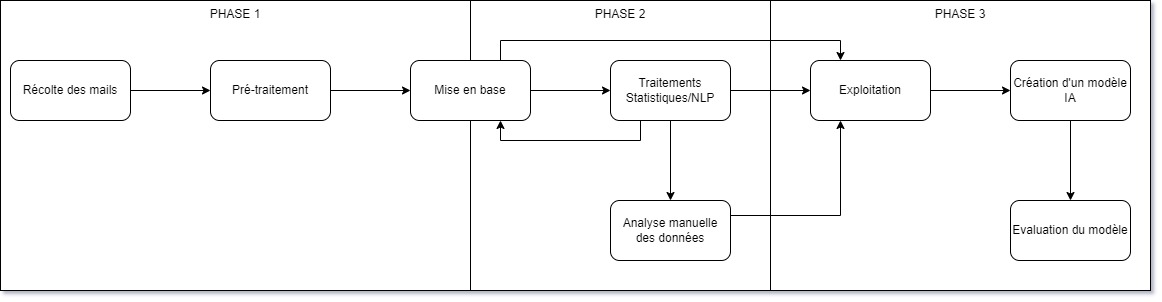
\includegraphics[width=\linewidth]{img/SchemaGeneral}
	\caption{Schéma des grandes étapes}
	\label{fig:SchemaGeneral}
\end{figure}

\subsection*{Mise en place de l'infrastructure opérationnelle}
	L'architecture opérationnelle s'appuie sur des conteneurs docker.
	Plusieurs types de base de données sont mises en œuvre profiter des avantages de chacune.
	Les conteneurs peuvent être gérés à l'aide du fichier \emph{Makefile} via les commandes suivantes :
	\begin{itemize}
		\item \emph{make docker\_start} : pour créer ou démarrer l'infrastructure
		\item \emph{make docker\_stop} : pour arrêter les conteneurs
		\item \emph{make docker\_prune} : pour nettoyer l'infrastructure
	\end{itemize}

	La figure~\ref{fig:Docker} montre l'organisation de cette architecture ainsi que les documents nécessaires pour son montage.
	\begin{figure}[H]
		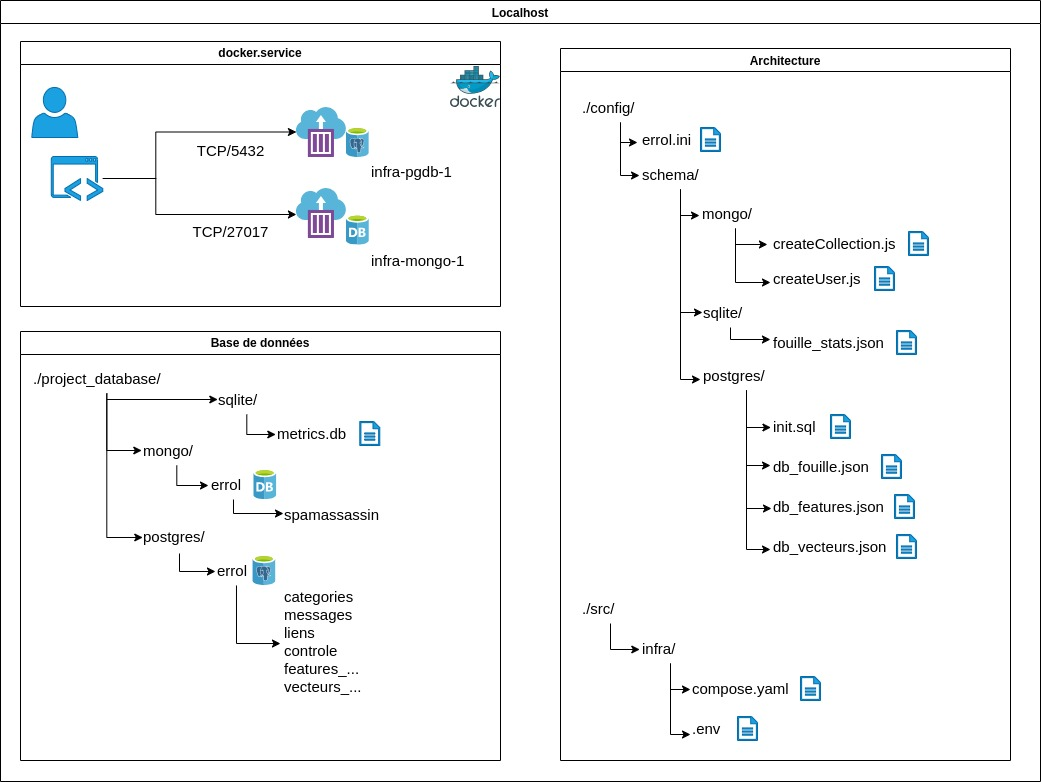
\includegraphics[width=\linewidth]{img/SchemaDocker}
		\caption{Schéma de l'architecture Docker}
		\label{fig:Docker}
	\end{figure}

	Les différentes tables et collections sont créées dynamiquement au cours des étapes du projet.

	\subsubsection*{Choix technologiques}
		\paragraph{Socle des services} 
			\subparagraph{Conteneurs}
				La conteneurisation des services permet d'effectuer facilement une séparation entre les processus.
				Les ressources empruntées à la machine hôte sont réduites au strict besoin de l'application.
				Une fois le moteur installé les différentes applications ou services peuvent être déployé rapidement.
				Chaque application embarque dans son conteneur toutes ses dépendances.
				Par définition les conteneurs sont volatils, des configurations complémentaires doivent être mises en place pour permettre la persistence des informations des bases de données.
				Solution retenue. \\
				Le moteur \emph{Docker} a été retenu, car il est simple d'utilisation, bien documenté et disponible sur plusieurs systèmes d'exploitation.
				Il est possible d'utiliser la capacité \emph{compose} de Docker pour déployer, démarrer ou arrêter plusieurs instances de manière coordonnée.

			\subparagraph{systemd}
				Une solution susceptible de fonctionner aurait été d'installer directement sur ma machine les différents services requis.
				Cela étant, un long processus d'installation puis de désinstallation aurait été nécessaire, avec le risque d'omettre des composants.
				De plus l'ajout de service directement sur la machine hôte comporte toujours des risques d'isolation des processus.
				Solution non retenue.

			\subparagraph{Machine virtuelle}
				L'installation des couches applicatives aurait pu être réalisé sur des machines virtuelles pour garantir une bonne isolation.
				Cela aurait également permit de simuler une infrastructure lourde avec plusieurs serveurs.
				Cependant, mon PC n'est pas en mesure de supporter l’exécution de plusieurs machines virtuelles en parallèle.
				Solution non retenue.

		\paragraph{Base NoSQL}
				Les bases de données NoSQL orientés documents sont plus performantes pour le stockage et l'accès à des ressources textuelles.
				Deux moteurs ont été testés :
			\subparagraph{MongoDB}
				Moteur de base données flexible et raisonnable en utilisation de ressource.
				Le langage des requêtes est simple à prendre en main.
				L'utilisation avec Python est facilitée par le \emph{Python developer path} disponible sur le site de l'éditeur.
				Solution retenue.

			\subparagraph{ElasticSearch}
				Moteur puissant de base de données qui intègre un moteur Lucène pour la recherche de document par mot clé.
				L'interface graphique associée (Kibana) est agréable et facile à prendre en main.
				Néanmoins, ce moteur est très gourmand en ressource.
				Une fois l'index (schéma) créé, il est très compliqué de le modifier.
				Solution rejetée.

		\paragraph{Base SQL}
			Les bases de données SQL sont plus performante quand il s'agit de traiter des informations transactionnelles.
			Elles offrent également plus de garantie de sécurité des données que les bases de données NoSQL\@.
			Elles permettent aussi de faire plus facilement et rapidement des requêtes complexes avec jointure et agrégation.
			Pour ces raisons, ce type de moteur sera utilisé pour stocker les informations numériques générées à partir des textes.
			\subparagraph{SQLite}
				Moteur de base de données SQL intégré avec Python.
				Les informations sont stockées dans un fichier défini.
				Cette base de données ne nécessite pas d'installer un service supplémentaire.
				Cette solution est généralement utilisée en phase de test.
				L'utilisation de cette solution pour stocker les données numériques des documents aurait été susceptible de générer des fichiers trop lourds et trop difficile à lier entre eux.
				Cependant, cette solution a été utilisée pour stocker les données générées lors de la phase de récolte (nombre de mails, nombre de mots uniques\ldots).
				Solution retenue

			\subparagraph{Postgres SQL}
				Moteur de base de données SQL solide et robuste.
				Elle permet également une gestion des utilisateurs ayant accès aux informations.
				L'intégration avec python est simple.
				Les données sont accessibles et peut être liées facilement.
				La taille des fichiers est gérée directement par le moteur.
				Solution retenue.
		\newpage

	\section{Fouille de données}
		\label{sec:fouille-de-donnees}
		Cette partie vise à expliquer les actions réalisées en vue de récupérer et stocker les données utilisées dans ce projet.
Au cours de cette phase plusieurs traitements permettront de réduire la quantité d'information pour se concentrer sur les corps des mails.
Les données MIME non textuelles sont écartés ainsi que les messages corrompus ou avec des encodages non convertibles en utf-8.

\subsection{Récolte des données}
	\paragraph{Recherche de dataset}
		Ma volonté initiale était de travailler sur des mails en français.
		Cependant, je n'ai pas trouvé de dataset dans cette langue.
		Je me suis donc retourné vers les dataset de mails en anglais. \\
		J'ai pu alors récupérer deux dataset :
			\begin{itemize}
				\item Enron company mails (voir~\ref{Enron_dataset})
				\item Dataset SpamAssassin (voir~\ref{SpamAssassin_dataset})
			\end{itemize}
			Les mails de SpamAssassin ont l'avantage d'être pré-trié, contrairement aux mails de la compagnie Enron.
			Ainsi le développement du moteur se fera uniquement avec les mails du SpamAssassin afin de pouvoir vérifier les résultats de l'analyse.

		\paragraph{Téléchargement des données}
			Le téléchargement du dataset Enron est possible à partir du moment où l'on possède un compte sur la plateforme Kaggle.
			Le dataset SpamAssassin est ouvert, il suffit de télécharger les archives de chaque catégorie. \\

			La récolte des données a été réalisée à la main sans automatisation.
			Les mails sont alors stockés dans plusieurs répertoires \emph{HAM} et \emph{SPAM} selon leur catégorie. \\

			Format :
			\begin{itemize}
				\item \emph{Enron} - 1 fichier CSV avec tous les mails
				\item \emph{SpamAssassin} - 1 fichier texte par mail
			\end{itemize}

	\paragraph{Evolution possible}
		La quantité de ressource disponible est assez limitée et principalement en anglais.
		Une idée aurait pu être de mettre en place un site internet où les utilisateurs peuvent fournir leurs mails avec la catégorie qu'ils estiment être la bonne. \\
		Cette solution comporte des points d'attentions.
		La confiance en l'utilisateur ne peut pas être absolue.
		Le rapport entre les ham et spam sera très probablement disproportionné en faveur des spams.
		Au vu des traitements effectués, cette solution nécessitera une gestion des données personnelles en accord avec les RGPD\@.

\subsection{Pré-traitement}
	La Figure~\ref{fig:Phase1} montre l'enchainement des étapes de traitement du mail puis du corps de texte jusqu'à la mise en base.
	Le chargement des mails en mémoire utilise le module python email (natif).
	Une grande partie des transformations sont effectuées en utilisant des expressions régulières.
	Trois points de contrôle permettent de décider si un mail sera effectivement utilisé ou non.
	\begin{enumerate}
		\item Échec de l'importation (fichier manquant lors de la tentative de lecture)
		\item Échec de récupération du corps (charset non accepté, corps vide, type du mail non textuel)
		\item Échec lors de la détermination de la langue (incapacité d'identifier les ngrams nécessaire à l'analyse)
	\end{enumerate}

	\begin{figure}[H]
		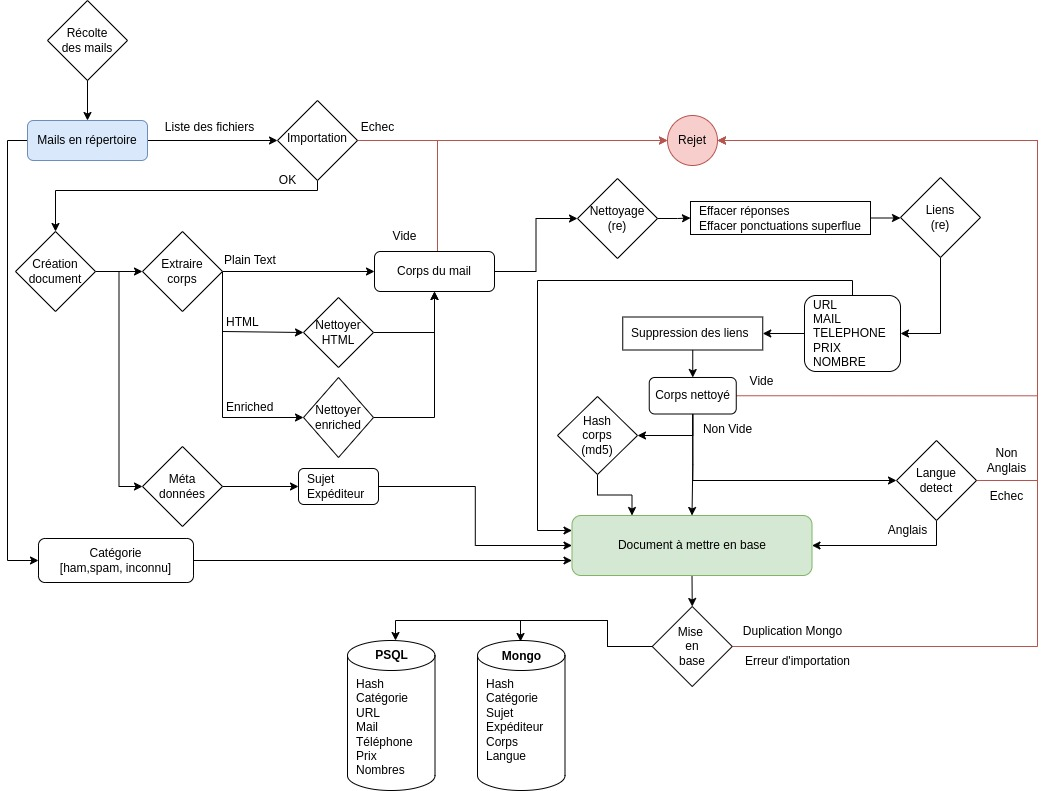
\includegraphics[width=\linewidth]{img/SchemaPhase1}
		\caption{Schéma des étapes de la phase 1}
		\label{fig:Phase1}
	\end{figure}

	\subsubsection{Importation}
		La fonction \emph{email.message\_from\_binary\_file} permet de transformer un fichier mail en objet python manipulable :
		\begin{lstlisting}[title=Fonction d'importation des fichiers,label={lst:import_file}]
def load_mail(file):
    with open(file, 'rb') as f_bin:
        return email.message_from_binary_file(f_bin)
		\end{lstlisting}

    \subsubsection{Extraction du corps des mails}
		Une fois le fichier importé au format \emph{EmailMessage}, il est possible d'en extraire le corps.
		Le corps du mail peut être composé de plusieurs parties qui ne sont pas forcément du texte.
		Les parties non textuelles ne sont pas conservée.

		\begin{lstlisting}[title=Extraction du corps du mail,label={lst:extract_corps}]
def extract_body(msg):
    refused_charset = ['unknown-8bit', 'default', 'default_charset',
                       'gb2312_charset', 'chinesebig5', 'big5']
    body = ""

    if msg.is_multipart():
        for part in msg.walk():
            if not part.is_multipart():
                body += extract_body(part)
        return body

    if msg.get_content_maintype() != 'text':
        return ""

    if msg.get_content_charset() in refused_charset:
        return ""

    if msg.get_content_subtype() == 'plain':
        payload = msg.get_payload(decode=True)
        body += payload.decode(errors='ignore')

    if msg.get_content_subtype() == 'html':
        payload = msg.get_payload(decode=True)
        body += nettoyage.clear_html(payload.decode(errors='ignore'))

    if msg.get_content_subtype() == 'enriched':
        payload = msg.get_payload(decode=True)
        body += nettoyage.clear_enriched(payload.decode(errors='ignore'))

    return body
		\end{lstlisting}

	\subsubsection{Nettoyage}
		Le nettoyage du texte utilise principalement les expressions régulières pour retirer un maximum d'éléments indésirables dans le texte.
        J'utilise également 2 modules externes afin de traiter le code HTML et faire la détection des mails qui ne sont pas écrits en anglais.

		\paragraph{Par regex}
			J'utilise le module python \emph{re} pour réaliser les traitements suivants :
			\subparagraph{Suppression des réponses}
				Lorsque l'on répond à un mail, le texte du message précédent est conservé dans le corps du mail.
                Pour permettre la distinction avec les mails précédant le caractère $>$ est ajouté en début de ligne.
                Je retire toutes les lignes correspondant à des réponses afin de limiter les doublons dans les textes.

			\begin{lstlisting}[title=Nettoyage des réponses,label={lst:clear_resp}]
def clear_reply(texte):
    pattern = re.compile('^>.*$', flags=re.MULTILINE)
    return re.sub(pattern, '', texte)
            \end{lstlisting}

			\subparagraph{Suppression des ponctuations}
				Pour ne pas surcharger la base de données et pour se concentrer sur le texte, une grande partie des caractères de ponctuation seront retirés.
                L'idée est de se concentrer sur les ponctuations classiques (.,?!).

				\begin{lstlisting}[title=Nettoyage des ponctuations,label={lst:clear_ponct}]
pattern_ponct = re.compile(r'[*#\\-_=:;<>\[\]"\'~)(|/$+}{@%&\\]', flags=re.MULTILINE)
def clear_ponctuation(texte):
    return re.sub(pattern_ponct, '', texte)
                \end{lstlisting}

			\subparagraph{Suppression des balises pour les enriched text}
				Certaines parties du corps de mail sont de type \emph{enriched text}.
				Les balises ne sont pas pertinente dans notre analyse et sont donc retirées.

				\begin{lstlisting}[title=Nettoyage des balises enriched text,label={lst:clear_enriched}]
pattern_enriched = re.compile('<.*>')
def clear_enriched(texte):
    return re.sub(pattern_enriched, '', texte)
                \end{lstlisting}

			\subparagraph{Suppression des liens}
				La présence de certaines informations comment les liens URL, les adresses mails et les numéros de téléphone ne peuvent pas être utilisés dans l'analyse textuelle.
                Cependant, il peut être intéressant de conserver une trace de leur présence.
                Nous allons ainsi modifier ces liens qui seront comptabilisés avant d'être retirés du texte.

				\begin{lstlisting}[title=Nettoyage des liens,label={lst:clear_liens}]
pattern_mail = re.compile('[a-zA-Z0-9_.+-]+@[a-zA-Z0-9-]+\\.[a-zA-Z0-9-.]+')
pattern_url1 = re.compile(r'(http|ftp|https)?://([\w\-_]+(?:(?:\.[\w\-_]+)+))'
                          r'([\w\-.,@?^=%&:/~+#]*[\w\-@?^=%&/~+#])?', flags=re.MULTILINE)
pattern_url2 = re.compile(r'(\w+\.)+\w+', flags=re.MULTILINE)
pattern_tel1 = re.compile(r'\(\d{3}\)\d+-\d+')  # (359)1234-1000
pattern_tel2 = re.compile(r'\+\d+([ .-]?\d)+')    # +34 936 00 23 23

def change_lien(texte, liens):
    temp, liens['MAIL'] = re.subn(pattern_mail, '', texte)

    temp, liens['URL'] = re.subn(pattern_url1, '', temp)
    temp, nb = re.subn(pattern_url2, '', temp)
    liens['URL'] += nb

    temp, liens['TEL'] = re.subn(pattern_tel1, '', temp)
    temp, nb = re.subn(pattern_tel2, '', temp)
    liens['TEL'] += nb

    return temp
                \end{lstlisting}

			\subparagraph{Suppression des nombres}
				Comme pour les liens, les nombres sont comptabilisés et retirés.
                Je fais la distinction entre les nombres seuls et les nombres accompagnés de sigle monétaires.
                \begin{verbatim}
                    MONNAIE = '$£€'
                \end{verbatim}
				\begin{lstlisting}[title=Nettoyage des nombres,label={lst:clear_nombre}]
pattern_prix1 = re.compile(f'[{MONNAIE}]( )?\\d+([.,]\\d+)? ', flags=re.MULTILINE)
pattern_prix2 = re.compile(f' \\d+([.,]\\d+)?( )?[{MONNAIE}]', flags=re.MULTILINE)
pattern_nb = re.compile('\\d+')

def change_nombres(texte, liens):
    temp, liens['PRIX'] = re.subn(pattern_prix1, '', texte)
    temp, nb = re.subn(pattern_prix2, '', temp)
    liens['PRIX'] += nb

    temp, liens['NOMBRE'] = re.subn(pattern_nb, '', temp)

    return temp
                \end{lstlisting}

		\paragraph{Par module}
			Lors du processus de nettoyage, j'utilise deux modules externes plus performants que ce que j'aurais pu faire simplement avec des expressions régulières.
            L'un me permet de nettoyer le code HTML, l'autre de détecter la langue du message.

			\subparagraph{Suppression du code HTML}
				Certaines parties du corps du mail sont de type HTML\@.
                J'utilise le module \emph{BeautifulSoup} pour parser le code et récupérer le texte affiché.

			    \begin{lstlisting}[title=Nettoyage des nombres,label={lst:clear_html}]
from bs4 import BeautifulSoup

def clear_html(texte):
    brut = BeautifulSoup(texte, "lxml").text
    return brut
                \end{lstlisting}
            Au cours du traitement avec ce module, j'ai eu une mise en garde.
            \begin{verbatim}
MarkupResemblesLocatorWarning - The input looks more like a filename than markup.
You may want to open this file and pass the filehandle into Beautiful Soup
            \end{verbatim}
            Après analyse, il semblerait que ce message soit levé dans le cas ou le module ne parvient pas à détecter et à récupérer le code html.
            Dans le mail concerné \\(\emph{spamassassin/spam/00307.7ed50c6d80c6e37c8cc1b132f4a19e4d}) la partie marquée comme HTML est également encodée en base64.
            \begin{verbatim}
------=_NextPart_7HZmySBWvSemNjin8Kg9YAA
Content-Type: text/html;
        charset="big5"
Content-Transfer-Encoding: base64

PGh0bWwgeG1sbnM6dj0idXJuOnNjaGVtYXMtbWljcm9zb2Z0LWNvbTp2bWwiDQp4bWxuczpvPSJ1
cm46c2NoZW1hcy1taWNyb3NvZnQtY29tOm9mZmljZTpvZmZpY2UiDQp4bWxuczp3PSJ1cm46c2No
ZW1hcy1taWNyb3NvZnQtY29tOm9mZmljZTp3b3JkIg0KeG1sbnM9Imh0dHA6Ly93d3cudzMub3Jn
L1RSL1JFQy1odG1sNDAiPg0KDQo8aGVhZD4NCjxtZXRhIGh0dHAtZXF1aXY9Q29udGVudC1UeXBl
IGNvbnRlbnQ9InRleHQvaHRtbDsgY2hhcnNldD1CaWc1Ij4NCjxtZXRhIG5hbWU9UHJvZ0lkIGNv
...         \end{verbatim}

            \subparagraph{Sélection des mails en anglais}
                Lors de mes tests, je me suis rendu compte que certains mails n'étaient pas en anglais.
                J'ai donc trouvé le module \emph{langdetect} qui permet de détecter le langage utilisé dans un texte en utilisant un modèle \emph{Naïve Bayes} avec une précision de 99\% (voir \ref{langdetect}). \\
				Je conserve dans les données à mettre en base le langage détecté avec l'idée de pouvoir traiter plusieurs langues dans le futur. \\

				La détection de la langue est réalisée juste avant la mise en base Mongo.

				\begin{lstlisting}[title=Création d'un document,label={lst:create_doc}]
import langdetect

def create_document(mail, categorie):
    corp = mail_load.extract_body(mail)
    corp, liens = nettoyage.clear_texte_init(corp)
    sujet, expediteur = mail_load.extract_meta(mail)

    if not corp:
        return None

    try:
        lang = langdetect.detect(corp)
    except langdetect.lang_detect_exception.LangDetectException:
        return None

    if lang != 'en':
        return None

    if categorie.lower() not in ['spam', 'ham']:
        categorie = 'inconnu'

    doc = {
        'hash': hashlib.md5(corp.encode()).hexdigest(),
        'categorie': categorie.lower(),
        'sujet': sujet,
        'expediteur': expediteur,
        'message': corp,
        'langue': lang,
        'liens': liens
    }
    return doc
                \end{lstlisting}


        \paragraph{Exemple de traitement}
            La section suivante montre des exemples de traitement de la phase 1.

        \begin{lstlisting}[title=Traitement initial,label={lst:clear_example_1}]
message = '''
Message dedicated to be a sample to show how the process is clearing the text.

Begin reply :
> He once said
>>> that it would be great
End of reply.

Substitutions :
spamassassin-talk@example.sourceforge.net
https://www.inphonic.com/r.asp?r=sourceforge1&refcode1=vs3390
hello.foo.bar
between $ 25 and 25,21 $

A number is : 2588,8 588
Phone type a : (359)1234-1000
Phone type b : +34 936 00 23 23
Ponctuation : ----## ..
~ ~~~~~
'''
text, liens = clear_texte_init(message)
print(liens)
print(text)
        \end{lstlisting}

        Résultat traitement initial :
        \begin{verbatim}
{'URL': 2, 'MAIL': 1, 'TEL': 2, 'NOMBRE': 3, 'PRIX': 2}

Message dedicated to be a sample to show how the process is clearing the text.

Begin reply


End of reply.

Substitutions



between and

A number is  ,
Phone type a
Phone type b
Ponctuation   ..
        \end{verbatim}

        \begin{lstlisting}[title=Traitement HTML,label={lst:clear_example_html}]
message_html = '''
<!DOCTYPE html PUBLIC "-//W3C//DTD HTML 4.01 Transitional//EN">
<html>
<head>
  <title>Foobar</title>
</head>
<body>
I actually thought of this kind of active chat at AOL
bringing up ads based on what was being discussed and
other features
  <pre wrap="">On 10/2/02 12:00 PM, "Mr. FoRK"
  <a class="moz-txt-link-rfc2396E"href="mailto:fork_
  list@hotmail.com">&lt;fork_list@hotmail.com&gt;</a>
  wrote: Hello There, General Kenobi !?
<br>
</body>
</html>
'''
print(clear_html(message_html))
        \end{lstlisting}
        Résultat traitement HTML :
        \begin{verbatim}

Foobar


I actually thought of this kind of active chat at AOL
bringing up ads based on what was being discussed and
other features
  On 10/2/02 12:00 PM, "Mr. FoRK"
  <fork_list@hotmail.com>
  wrote: Hello There, General Kenobi !?


        \end{verbatim}

        \begin{lstlisting}[title=Traitement enriched text,label={lst:clear_example_enriched}]
message_enriched = '''
<smaller>I'd like to swap with someone also using Simple DNS to take
advantage of the trusted zone file transfer option.</smaller>
'''
print(clear_enriched(message_enriched))
        \end{lstlisting}

        Résultat traitement enriched text :
        \begin{verbatim}
I'd like to swap with someone also using Simple DNS to take
advantage of the trusted zone file transfer option.
        \end{verbatim}


\subsection{Mise en base}
    La mise en base et le dernier traitement de cette phase.
    Les traitements précédents ont créé une liste de dictionnaires python contenant les valeurs à sauvegarder (document).
    Chaque document répond au schéma défini dans le tableau~\ref{tab:mapping_fouille} \\
    \begin{table}[H]
        \centering
        \begin{tabular}{lccr}
            Clé & Mongo & PSQL & Description\\
            \hline
            hash & \_id & messages(hash) & signature md5 du corp\\
            categorie & categorie & categories(nom) & ham, spam, inconnu\\
            sujet & sujet & & sujet du mail\\
            expediteur & expediteur & & source du mail\\
            message & message & & corps du mail\\
            langue & langue & & en\\
            liens['URL'] & & liens(url) & nombre d'url\\
            liens['MAIL'] & & liens(mail) & nombre d'adresses mail\\
            liens['TEL'] & & liens(tel) & nombre de numéros de téléphone\\
            liens['PRIX'] & & liens(prix) & nombre de références à des prix\\
            liens['NOMBRE'] & & liens(nombre) & nombre d'apparitions de nombres\\
            \hline
        \end{tabular}
        \caption{Mapping des clés python avec les bases de données}
        \label{tab:mapping_fouille}
    \end{table}

    La valeur du hash va permettre d'exclure les doublons qui ont déjà été insérés dans les bases MongoDB et PSQL\@.
    Cette valeur va également permettre de faire la liaison entre les données des différentes bases.\\
    Le schéma~\ref{fig:BddPhase1} illustre l'état des relations entre les bases de données PSQL et Mongo.

    \begin{figure}[H]
		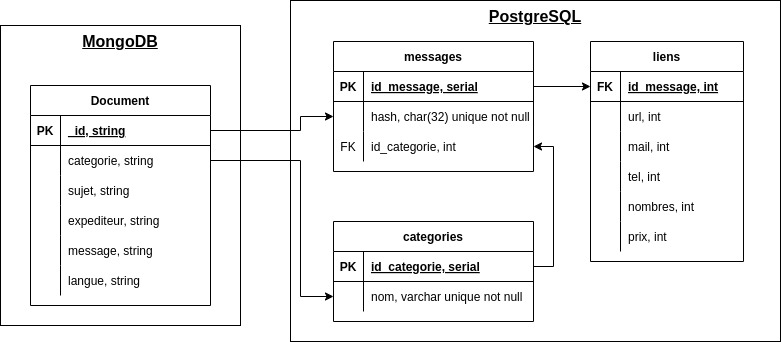
\includegraphics[width=\linewidth]{img/bddFouille}
		\caption{Relation entre les bases de données}
		\label{fig:BddPhase1}
	\end{figure}

    \paragraph{Wrapper en python}
        La communication entre le programme et les bases de données se fait au moyen des modules suivants :
        \begin{itemize}
            \item[-] MongoDB - pymongo (bibliothèque officielle maintenue par mongoDB)
            \item[-] PSQL - psycopg2 (bibliothèque open-source), utilisée pour les requêtes simples
            \item[-] PSQL - sqlalchemy (bibliothèque open-source), utilisée pour les requêtes complexes
            \item[-] SQLite - sqlite3 (bibliothèque standard de python)
        \end{itemize}

        Des modules internes au programme ont été développer pour simplifier l'utilisation des modules d'interaction avec les bases de données.
        Les packages cmd\_mongo.py, cmd\_psql.py, cmd\_sqlite.py regroupent les fonctions qui sont utilisées pour les intéractions entre le programme et les bases respectives.

    \paragraph{Problèmes éventuels}
        Lors de l'insertion les cas suivants sont susceptibles d'arriver si les deux bases n'ont pas été correctement nettoyées.\\
        \begin{table}[H]
            \centering
            \begin{tabular}{|p{4cm}|p{4cm}|p{7cm}|}
                \hline
                Situation & Raison & Solution\\
                \hline
                Mail présent dans Mongo et absent dans PSQL & Échec d'insertion dans la base PSQL & Supprimer l'entrée dans la base Mongo et relancer le traitement pour ce mail\\
                \hline
                Mail présent dans PSQL et absent dans Mongo & Suppression du mail dans la base Mongo & Supprimer le mail et toutes ses références dans la base PSQL et relancer le traitement de ce mail\\
                \hline
            \end{tabular}
            \caption{Problèmes possibles avec la mise en base}
            \label{tab:pb-base}
        \end{table}


    \paragraph{Stockage des données statistiques du traitement - SQLite}
        Les données présentent dans cette base permettent de suivre l'évolution de certaines métriques lors des différentes étapes du nettoyage.
        Lors de chaque étape de la phase 1 (Récolte, Création des documents, Mise en base), je calcule pour les HAM, SPAM et (HAM+SPAM) les éléments suivants :
        \begin{itemize}
            \item[-] mails - nombre de mails
            \item[-] mots - nombre de mots dans tout le corpus
            \item[-] mots\_uniques - nombre de mots uniques dans tout le corpus
        \end{itemize}

        Ces données me permettent d'estimer la quantité de données nettoyées durant cette phase.

        \begin{figure}[H]
            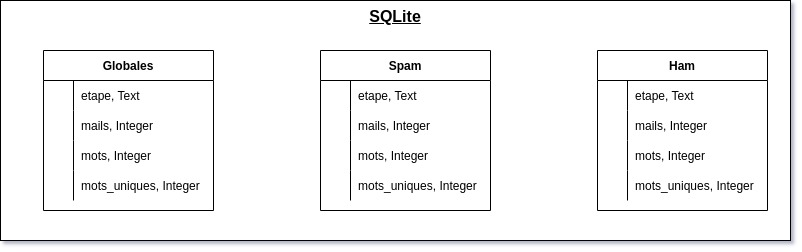
\includegraphics[width=\linewidth]{img/Schemasqlite}
            \caption{Schéma de la base de données pour lors du traitement}
            \label{fig:sqlite_schema}
        \end{figure}

\subsection*{Analyse}
    L'exécution du programme donne les informations présentées dans le tableau~\ref{tab:fouillestats}.
    \begin{table}[H]
        \centering
        \begin{tabular}{l|rrr|rrr|rrr}
            & \multicolumn{3}{c}{mails} & \multicolumn{3}{c}{mot} & \multicolumn{3}{c}{mots uniques}\\
            étapes & globale & spam & ham & globale & spam & ham & globale & spam & ham\\
            \hline
            récolte & 5798 & 1897 & 3901 & 2385120 & 916756 & 1468364 & 262614 & 129090 & 133524\\
            création & 5662 & 1786 & 3876 & 1223062 & 589364 & 633698 & 99837 & 40676 & 59161\\
            mise en base & 5334 & 1530 & 3804 & 1163777 & 533686 & 630091 & 99834 & 40676 & 59158\\
        \end{tabular}
        \caption{Données statistiques de la fouille}
        \label{tab:fouillestats}
    \end{table}
    
    La figure~\ref{fig:dashFouille} montre un aperçu des données statistiques récoltées durant cette première phase.
    Les 3 premiers graphiques montrent l'évolution du nombre de documents, de mots et de mots uniques en fonction des étapes intermédiaires.\\
    Cette visualisation permet de faire les observations suivantes :
    \begin{itemize}
        \item[-] La diminution des documents spam est plus importante que celle des ham
		\item[-] Le nombre de mots uniques ne diminue plus après la création de document
		\item[-] La diminution du nombre de mots est plus importante dans les ham que dans les spam
		\item[-] Le nombre de mots uniques est plus important dans les ham que dans les spam
    \end{itemize}
    Après la phase de récolte, on remarque qu'il y a un nombre plus important de document en double dans la catégorie \emph{spam}.
    Il y a également une réduction importante du nombre de mots ainsi que du nombre de mots uniques dans les \emph{ham}.
    Cette réduction peut s'expliquer par le nettoyage du corps des mails :
    \begin{itemize}
        \item Retrait des réponses
        \item Retrait de certaines ponctuations
        \item Suppression des balises HTML et enriched text
        \item Retrait des liens, et nombres
    \end{itemize}

    Enfin, on peut voir que les \emph{ham} utilisent plus de mots uniques que les \emph{spam}.
    Il est donc possible que le vocabulaire des \emph{spam} soit plus restreint.
    \begin{figure}[H]
        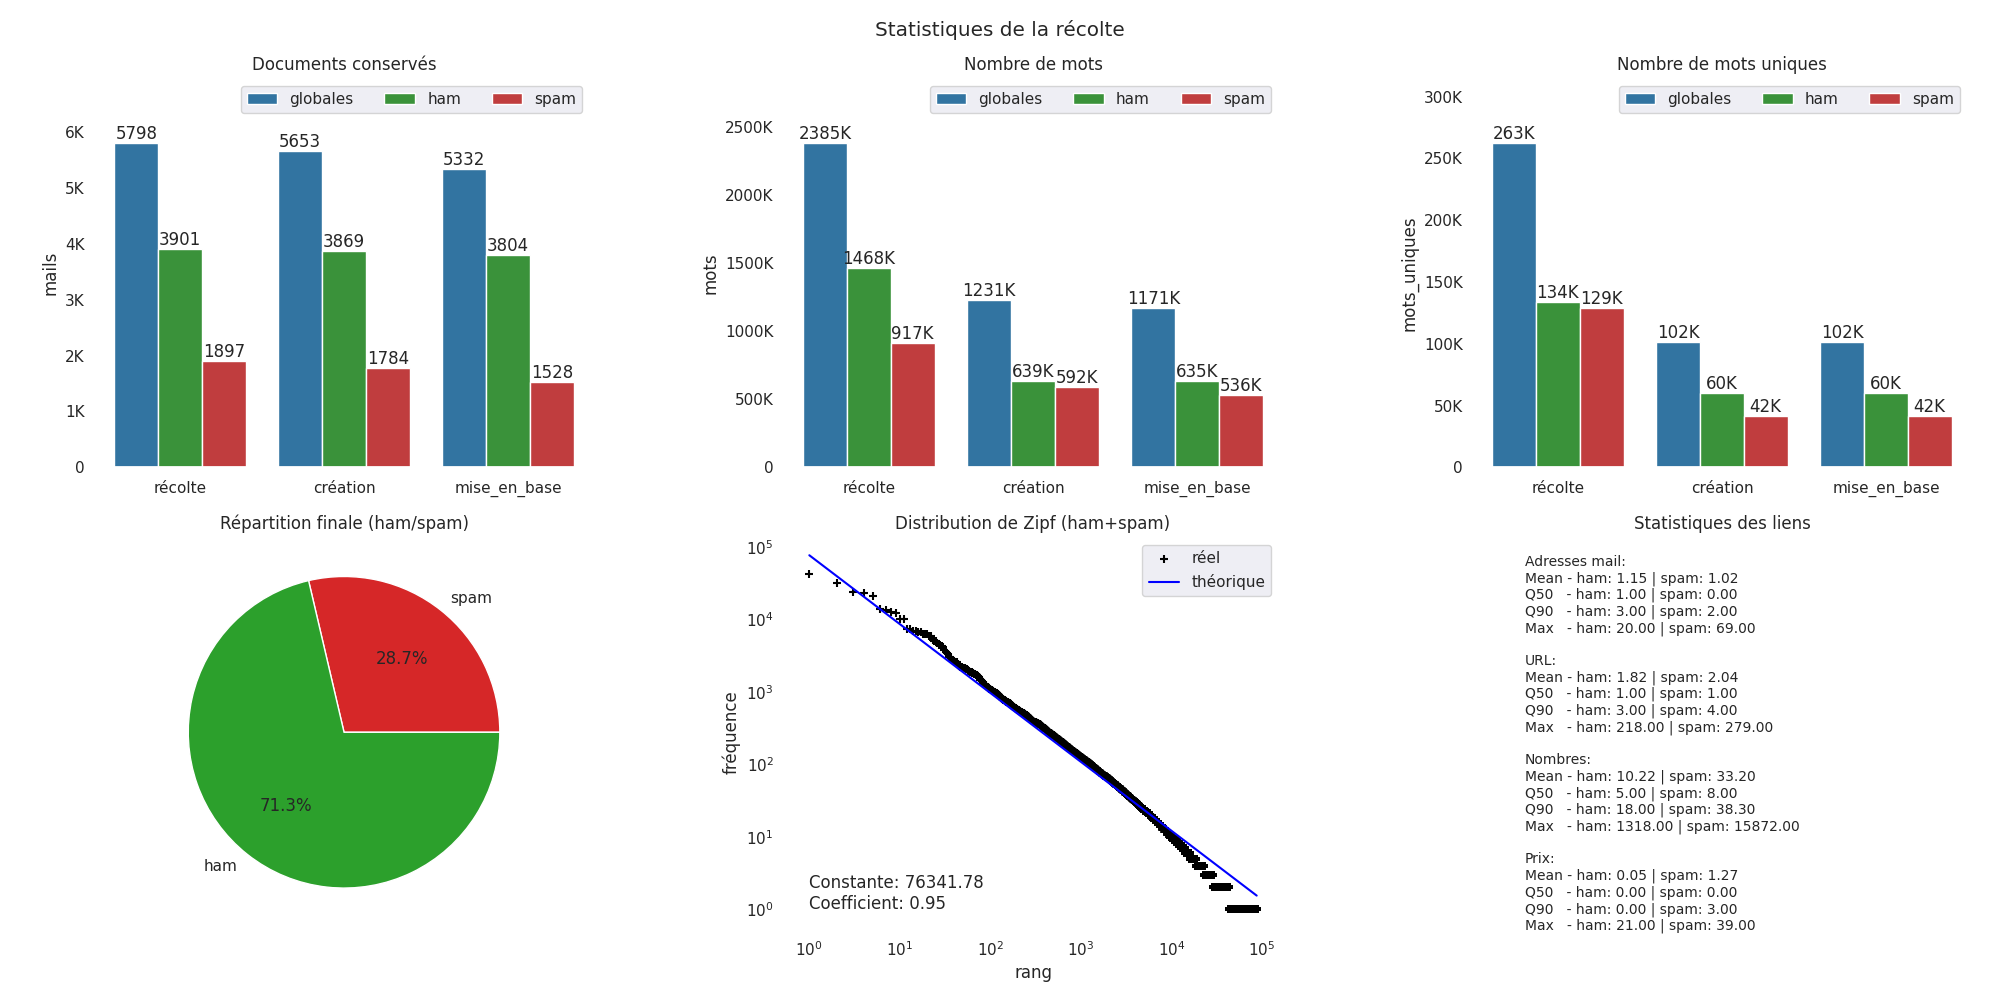
\includegraphics[width=\linewidth]{img/fouilleStats}
        \caption{Tableau de bord de la fouille}
        \label{fig:dashFouille}
    \end{figure}

    À l'issue de ces traitements, la proportion dans notre dataset ham/spam est d'environ 70/30.
    On voit aussi que la distribution du Zipf est globalement respectée.
    Il est ainsi fortement probable que notre dataset respecte les caractéristiques linguistiques naturelles.\\

    L'extraction des liens informations numériques donne les statistiques du tableau~\ref{tab:p1liens}.
    \begin{table}[H]
        \centering
        \begin{tabular}{l|rr|rr|rr|rr|rr}
            & \multicolumn{2}{c}{url} & \multicolumn{2}{c}{mail} & \multicolumn{2}{c}{tel} & \multicolumn{2}{c}{prix} & \multicolumn{2}{c}{nombre}\\
            & spam & ham & spam & ham & spam & ham & spam & ham & spam & ham\\
            \hline
            moyenne & 5.25 & 3.83 & 1.01 & 1.13 & 0.06 & 0.20 & 0.81 & 0.03 & 30.36 & 7.1\\
            médiane & 3 & 2 & 0 & 1 & 0 & 0 & 0 & 0 & 7 & 4\\
            90\% & 9 & 6 & 2 & 3 & 0 & 1 & 2 & 0 & 35 & 14\\
            maximum & 295 & 470 & 69 & 20 & 67 & 25 & 29 & 17 & 15801 & 731\\
        \end{tabular}
        \caption{Statistiques sur les liens et informations numériques}
        \label{tab:p1liens}
    \end{table}
    Les données statistiques sur les liens ne permettent pas mettre en avant une différence franche dans l'utilisation de ces éléments dans les catégories observées.
    Seul la présence de nombres ou d'URL seraient éventuellement susceptible d'apporter une aide à la catégorisation.


\subsection*{Choix techniques}
    \paragraph{Langage de programmation}
        Python a été choisi pour développer ce programme pour les raisons énoncées ci-dessous :
        \begin{itemize}
            \item[-] Large choix de modules, dont plusieurs spécialisés dans le traitement de données
            \item[-] Langage simple et flexible
            \item[-] Facilement portable et executable avec la fourniture des environnements virtuel
        \end{itemize}

    \paragraph{Métriques}
        L'utilisation du nombre de documents, de mots et de mots uniques pour mesurer la performance de cette phase a été commandée par le cours.
        Il n'y a pas eu de difficultés majeures sur cette partie.
        Ces données ne sont pas conservées au fur et à mesure des diverses importations.
        Je n'ai pas jugé pertinent de les employer lors des traitements futurs. \\

        La recherche des apparitions d'adresse mail, de liens url, de numéros de téléphone, de prix et de nombres est une idée personnelle.
        Je voulais voir si ces éléments étaient susceptible d'être discriminant pour la classification.
        Les résultats ne sont pas aussi marqués que je ne l'aurais cru.
        Je pense qu'il aurait été possible d'améliorer la justesse de ces données en travaillant sur plus de cas possible.
        Ou en analysant plus en profondeur les substitutions effectuées notamment sur les nombres.\\
        Cela étant la substitution et effacement de ces éléments dans le corps de texte peut répondre à une nécessité d'anonymisation.
        De plus la suppression des liens URL évite de conserver et de rendre accessible des liens potentiellement frauduleux.\\

        Le développement du code pour la distribution de ZIPF a été réalisée suite à une discussion avec le professeur.
        Initialement, je souhaitais également tester cette distribution sur chaque message individuellement.
        Mais la quantité de mots par message n'est peut-être pas suffisant pour obtenir des résultats probants.
        J'ai dû me renseigner beaucoup pour arriver à comprendre l'équation sous-jacente et comment je pouvais la coder de manière efficace et visuelle.
        Vous pouvez voir le résultat de ce travail dans l'annexe~\ref{sec:devZipf}.

\newpage
\subsection*{Exemple du programme de fouille}
    \begin{verbatimtab}
$ make venv
$ make docker_start
cd ./src/infra/; docker compose up -d
[+] Running 3/3
 ✔ Network infra_default    Created                                                                                                                                                                           0.1s
 ✔ Container infra-mongo-1  Started                                                                                                                                                                           0.5s
 ✔ Container infra-pgdb-1   Started

$ source .venv/bin/activate
(.venv)$ ./errol.py fouille -g \
        -a ./project_data/spamassassin/easy_ham \
           ./project_data/spamassassin/easy_ham_2 \
        -p ./project_data/spamassassin/spam \
           ./project_data/spamassassin/spam_2
    \end{verbatimtab}

    Il est possible d'accéder aux bases de données avec les commandes suivantes:
    \begin{verbatimtab}
$ sqlite3 project_database/sqlite/metrics.db
$ psql -h localhost -p 5432 errol psql_errol
$ mongosh -u mongo_errol -p <MOT DE PASSE> errol
    \end{verbatimtab}
		\newpage
	
	\section{Ingénierie des langues}
		\label{sec:ingenierie-des-langues}
		Les opérations de cette phase ont pour but d'extraire les caractéristiques des textes collectés à la phase précédente.
Nous allons rechercher des informations numériques sur la forme des messages comme le nombre de mots, de ponctuations, \ldots\\
Enfin, nous appliquerons des techniques de traitement du langage naturel pour travailler sur le fond des corps de mail.


\subsection{Recherche de caractéristiques}
    Durant cette phase, nous allons rechercher les caractéristiques de la forme du texte.
    L'objectif est de voir si l'utilisation de ponctuation, de certaines formes de mots (majuscule/minuscule)
    ou de construction visuelle d'un texte (espace ligne) est différente pour chaque catégorie de mail.\\

    Les messages seront directement extraits de la base mongo utilisée lors de la phase de fouille.
    Chaque message sera analysé individuellement dans une suite de fonction.
    Les étapes de cette phase sont décrites dans le schéma~\ref{fig:Phase2}.

    \begin{figure}[H]
        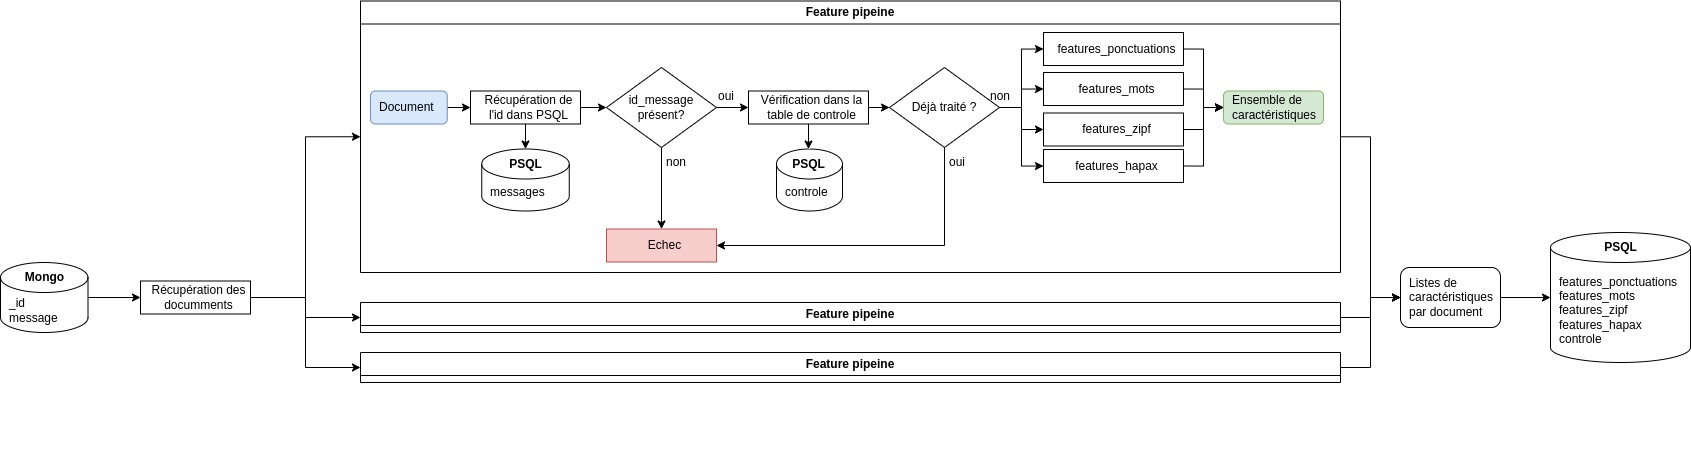
\includegraphics[width=\linewidth]{img/features}
        \caption{Schéma de la recherche de caractéristiques}
        \label{fig:Phase2}
    \end{figure}



    \begin{lstlisting}[title=Fonctions de la recherche de caractéristiques,label={lst:feat_func}]

def features_ponctuations(texte):
    return {
        "point": texte.count('.'),
        "virgule": texte.count(','),
        "exclamation": texte.count('!'),
        "interrogation": texte.count('?'),
        "tabulation": texte.count('\t'),
        "espace": texte.count(' '),
        "ligne": texte.count('\n') + 1,
        "ligne_vide": len(re.findall(r'^\s*$', texte, re.MULTILINE))
    }

ef features_mots(texte):
    tokens = re.findall(r'\w+', texte, re.MULTILINE)
    return {
        'char_minuscules': len(re.findall(r'[a-z]', texte, re.MULTILINE)),
        'char_majuscules': len(re.findall(r'[A-Z]', texte, re.MULTILINE)),
        'mots': len(tokens),
        'mots_uniques': len(set(tokens)),
        'mots_majuscules': sum(mot.isupper() for mot in tokens),
        'mots_capitalizes': sum(bool(re.match(r'[A-Z][a-z]+', mot)) for mot in tokens)
    }


def features_zipf(texte):
    tokens = re.findall(r'\w+', texte, re.MULTILINE)
    z_data = zipf.zipf_process(tokens)
    return {
        'constante': float(z_data.get('const_moy')),
        'coefficient': float(z_data.get('coef_min')),
        'taux_erreur': float(z_data.get('cout_min'))
    }


def features_hapax(texte):
    tokens = re.findall(r'\w+', texte, re.MULTILINE)
    data = zipf.hapax(tokens)
    data['nombre_hapax'] = data.pop('nombres')
    return data
    \end{lstlisting}

    \subsubsection*{Choix technologiques}
        \paragraph{Traitements}
            La recherche des caractéristiques de ponctuations, de type de char, ou de lignes est faite en utilisant la fonction
            standard \emph{str.count()} et le module \emph{re}.\\

            Cette suite de traitement intègre également des fonctions pour le calcul de la distribution de Zipf (annexe~\ref{sec:devZipf}).
            Cela étant, il est possible que les messages soient trop court pour que ces fonctions donnent des résultats pertinents.\\

            L'ensemble des messages sont récupérés dans la base mongo en une seule fois avec l'\_id correspondant au hash.
            Le traitement est effectué sur chaque document en utilisant le module multiprocessing.

        \paragraph{Base de données}
            Les données des documents sont stockées dans des nouvelles tables PSQL initialisées au début du programme.
            Le nouveau schéma PSQL est montré dans la figure \ref{fig:feat_db}
            Cette base a été choisie pour bénéficier des capacités d'insertion par lots et de jointure offertes par SQL\@.
            Plusieurs tables sont ajoutées en liaison avec nom de la fonction de traitement.
            Les tables ajoutées :
            \begin{itemize}
                \item features\_hapax
                \item features\_mots
                \item features\_ponctuations
                \item features\_zipf
            \end{itemize}
            \begin{figure}[H]
                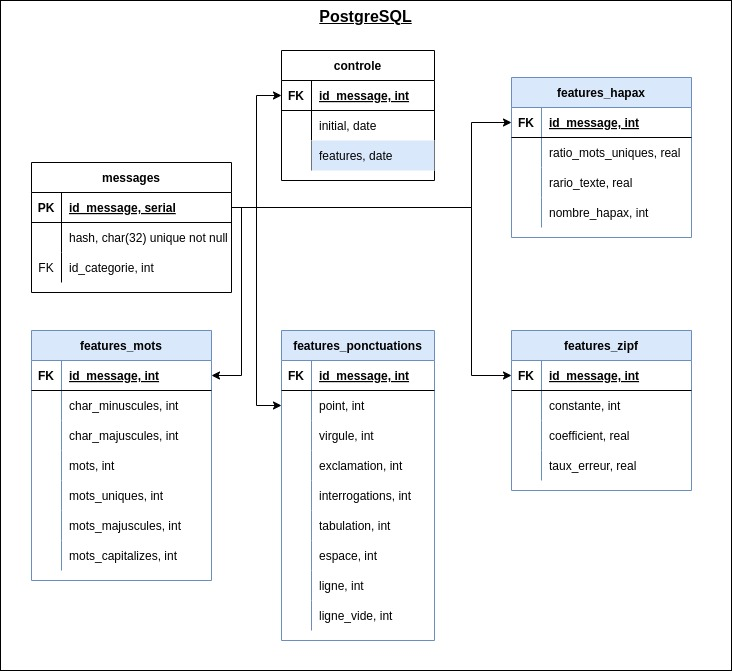
\includegraphics[width=\linewidth]{img/features_bdd}
                \caption{Schéma de la base pour la recherche de caractéristiques}
                \label{fig:feat_db}
            \end{figure}

    \subsubsection*{Analyse partielle}
    TODO

\subsection{Traitement du langage}
    Dans cette section, nous aborderons les traitements du langage naturel qui vont être employés afin de tenter de
    détecter des similitudes dans les thèmes abordés dans les mails de chaque catégorie.
    Nous allons transformer les messages en un dictionnaire de mot et de fréquence.
    Les données récoltées seront utilisées pour vectoriser les documents avec la méthode TF-IDF\@.

    \subsubsection{Lemmatisation}
        La lemmatisation d'un texte vise à réduire la taille d'un texte en ramenant chaque mot à la forme du mot présente dans le dictionnaire.
        Ce traitement permet donc de compter le nombre d'occurrences d'un mot sans se soucier de sa forme ou des modifications grammaticales appliquées lors de la rédaction du texte.
        A l'issue de ce traitement, nous serons en mesure de connaître les mots les plus utilisés dans les corps des mails et tenter de déterminer les thèmes les plus récurrents.
        Dans ce projet, nous allons utiliser le moteur de lemmatisation de \emph{StandfordNLP}\cite{manning-EtAl:2014:P14-5}\cite{qi2020stanza}
        Les traitements nécessaire pour arriver à une lemmatisation sont :
        \begin{enumerate}
            \item Tokenisation - Séparer les phrases en token. Ici chaque token correspond à un mot ou à une ponctuation.
            \item Multi-Word Token Expansion - Ce traitement n'est pas nécessaire en anglais selon la documentation \emph{Stanza}. Il permet d'étendre un token s'il correspond à une contraction de plusieurs terme. Par exemple en français le terme \emph{du} sera transformé en \emph{de le}.
            \item Part of Speech Tagging - Cette opération vise à marquer chaque mot du texte avec sa position grammaticale dans la phrase qui le contient et va permettre d'effectuer le transfert vers le lexème correspondant.
        \end{enumerate}

        L'initialisation de la pipeline de lemmatisation de Stanza se fait en appelant la classe \emph{Pipeline} avec les arguments de langage et de processus dans l'ordre d'utilisation.
        A cette étape, j'ajoute 2 filtres.
        Le premier va me permettre de ne conserver que les mots avec des lettres.
        La deuxième étape permet de retirer les stopwords en anglais qui ne permettent pas d'analyser le sens du message.\\
        La dernière étape avant la mise en base permet de compter la fréquence de chaque mot dans le texte.
        Le schéma~\ref{fig:nlp} illustre l'enchainement des étapes de cette phase.

        \begin{lstlisting}[title=Pipeline de lemmatisation, language=python]
import nltk
import stanza
from src.annexes import zipf

nltk.download("stopwords")
en_stopwd = set(stopwords.words('english'))
pipe = stanza.Pipeline(lang='en', processors='tokenize,mwt,pos,lemma')
pat = re.compile(r'\w+')

def lemmatise(message, stopwds, pipeline, pattern):
    doc = pipeline(message)
    lemma = [mot.lemma for phrase in doc.sentences for mot in phrase.words]
    return [lem.lower() for lem in lemma if re.match(pattern, lem) and lem.lower() not in stopwds]

zipf.freq_mot(lemmatise(value, en_stopwd, pipe, pat))
			\end{lstlisting}

			Ci-dessous un exemple des étapes du traitement sur un message de la base
			\begin{verbatim}
>>> print(value)
Heres the hottest thing in DVDs. Now you can make a personal backup
copy of a DVD right onto CDR.  Our Hot new software easily takes you through
the steps to make a copy of your own DVDs.
NOW INCLUDED FOR FREE! Copy PLAYSTATION, MUSICMPs and all Software.
 Step by Step Interactive Instructions
 All Software Tools Included On CD
 No DVD Burner Required
 FREE Live Technical Support
  Day Risk Free Trial Available
 FREE Dvd Movie of your choice LIMITED TIME OFFER!
We have All the software you need to COPY your own DVD Movies.
This email has been screened and filtered by our in house OPTOUT system in
compliance with state laws. If you wish to OPTOUT from this mailing as well
as the lists of thousands  of other email providers please visit
ZKZmblanzxaDBmnTTIcorikgl

>>> lemmatise(value, en_stopwd, pipe, pat)
['hot', 'thing', 'dvd', 'make', 'personal', 'backup', 'copy', 'dvd', 'right', 'onto',
 'cdr', 'hot', 'new', 'software', 'easily', 'take', 'step', 'make', 'copy', 'dvd',
 'include', 'free', 'copy', 'playstation', 'musicmps', 'software', 'step', 'step',
 'interactive', 'instruction', 'software', 'tool', 'include', 'cd', 'dvd', 'burner',
 'require', 'free', 'live', 'technical', 'support', 'day', 'risk', 'free', 'trial',
 'available', 'free', 'dvd', 'movie', 'choice', 'limited', 'time', 'offer',
 'software', 'need', 'copy', 'dvd', 'movie', 'email', 'screen', 'filter', 'house',
 'optout', 'system', 'compliance', 'state', 'law', 'wish', 'optout', 'mailing',
 'well', 'list', 'thousand', 'email', 'provider', 'please', 'visit',
 'zkzmblanzxadbmntticorikgl']

>>> zipf.freq_mot(lemmatise(value, en_stopwd, pipe, pat))
{'hot': 2, 'thing': 1, 'dvd': 6, 'make': 2, 'personal': 1, 'backup': 1, 'copy': 4,
 'right': 1, 'onto': 1, 'cdr': 1, 'new': 1, 'software': 4, 'easily': 1, 'take': 1,
 'step': 3, 'include': 2, 'free': 4, 'playstation': 1, 'musicmps': 1,
 'interactive': 1, 'instruction': 1, 'tool': 1, 'cd': 1, 'burner': 1,
 'require': 1, 'live': 1, 'technical': 1, 'support': 1, 'day': 1, 'risk': 1,
 'trial': 1, 'available': 1, 'movie': 2, 'choice': 1, 'limited': 1, 'time': 1,
 'offer': 1, 'need': 1, 'email': 2, 'screen': 1, 'filter': 1, 'house': 1,
 'optout': 2, 'system': 1, 'compliance': 1, 'state': 1, 'law': 1, 'wish': 1,
 'mailing': 1, 'well': 1, 'list': 1, 'thousand': 1, 'provider': 1, 'please': 1,
 'visit': 1, 'zkzmblanzxadbmntticorikgl': 1}
			\end{verbatim}

    \begin{figure}[H]
        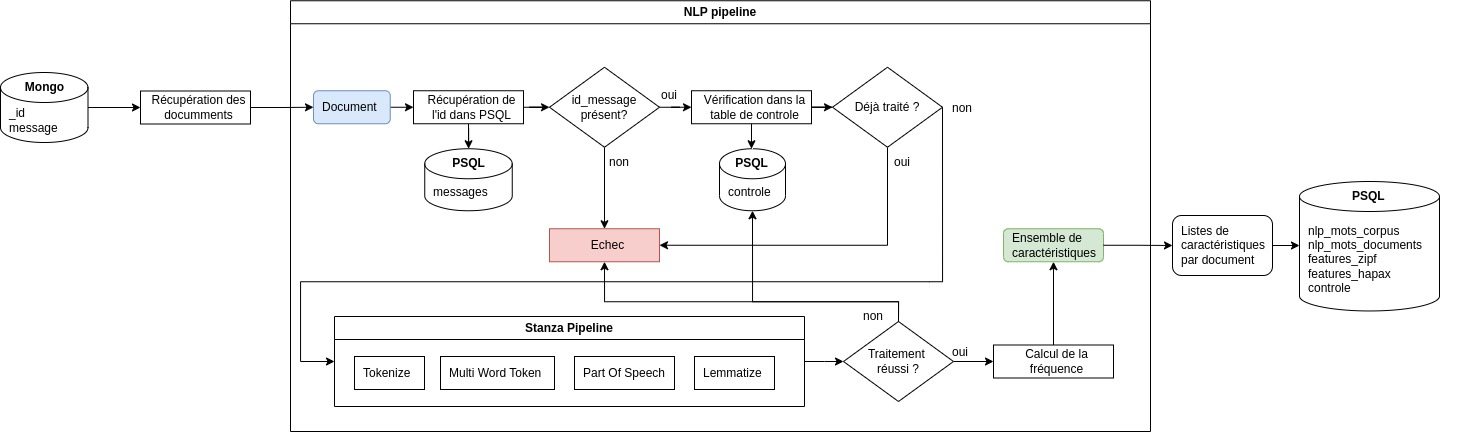
\includegraphics[width=\linewidth]{img/nlp}
        \caption{Schéma du traitement NLP}
        \label{fig:nlp}
    \end{figure}

    \paragraph{Erreurs possibles lors du traitement NLP}
    \begin{itemize}
        \item TypeError - Provient de la présence de données non textuelle dans le corps du mail (ex: MIME)
		\item OutOfMemoryError - Présence de mot beaucoup trop long pour être parsé.
	\end{itemize}

    \paragraph{Choix techniques}
        Seules les librairies de Stanza ont été utilisées pour ce projet pour le traitement de texte.
        J'ai apprécié la simplicité d'intégration de la pipeline dans le code.
        De plus Stanza intègre une capacité de MWT qui aurait pu être utile dans le cas de traitement des mails en français.
        D'autres concurrents sérieux auraient pu être NLTK et SpaCy. Je n'ai pas eu le temps de les approfondir.\\

        Dans cette phase l'utilisation du mutliprocessing n'a pas pu être mis en place à cause d'une RAM limitée qui aurait pu entrainer des échec de traitement.
        De plus, l'utilisation de torch.cuda par la pipeline Stanza nécessite trop d'ajustement au niveau du code pour être utilisées dans ce context.

    \paragraph{Base de données}
        Le schéma de la base de données PSQL pour cette phase est montrée dans la figure~\ref{fig:nlp_db}.
        La table de contrôle récupère 2 nouvelles colonnes
        \begin{itemize}
            \item nlp - date du traitement
            \item nlp\_status - résultat OK, Type error, Memory error
        \end{itemize}

        Deux nouvelles tables sont ajoutées pour stocker les informations nécessaires pour la vectorisation
        \begin{itemize}
            \item nlp\_mots\_corpus - liste des mots présents après les phases de traitement
            \begin{itemize}
                \item freq\_corpus - occurrences du mot dans tout le corpus
                \item freq\_documents - nombre de documents ayant au moins une occurrence de ce mot
                \item freq\_ham - nombre de ham ayant au moins une occurrence de ce mot
                \item freq\_spam - nombre de spam ayant au moins une occurrence de ce mot
            \end{itemize}
            \item nlp\_mots\_documents - liste d'association entre les mots et les documents.
            \begin{itemize}
                \item occurrence - fréquence d'un certain mot dans un document particulier
            \end{itemize}
        \end{itemize}

        \begin{figure}[H]
            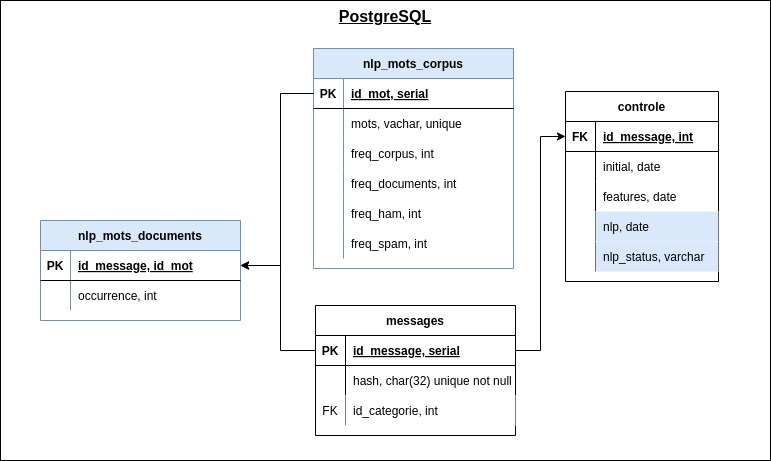
\includegraphics[width=\linewidth]{img/nlp_bdd}
            \caption{Schéma de la base pour le traitement du langage}
            \label{fig:nlp_db}
        \end{figure}

    \paragraph{Analyse partielle}
    TODO

	\subsubsection{Vectorisation}
	    La vectorisation d'un texte doit permettre de transposer les données textuelles en données numériques afin de
        pouvoir les utiliser dans des calculs statistiques ou dans les modèles d'apprentissage automatiques.\\
		J'ai choisi d'utiliser une vectorisation TF-IDF\cite{ml-python} (Term Frequency-Inverse Document Frequency).
        Cette méthode se rapproche de la distribution de Zipf détaillée précédemment.
        En effet, le score d'un terme est dépendant de la fréquence dans le document et de la fréquence de ce terme dans l'ensemble du corpus.
        La formule utilisée est :
        \begin{align*}
            W_{i,j} = tf_{i,j}*log(\frac{N}{df_{i}})
        \end{align*}

        Avec $tf_{i,j}$ la fréquence d'apparition du mot $i$ dans le document $j$, $N$ le nombre de documents dans le corpus et $df_{i}$ le nombre de documents dans le corpus contenant le terme $i$. \\
        Cette méthode permet d'attribuer un score plus élevé aux mots apparaissant plus dans un document que dans les autres documents du corpus.
        Nous pouvons ainsi conserver une forme de contexte d'utilisation.
        La figure~\ref{fig:tfidf} montre les étapes pour vectoriser l'ensemble des documents.

        \begin{figure}[H]
            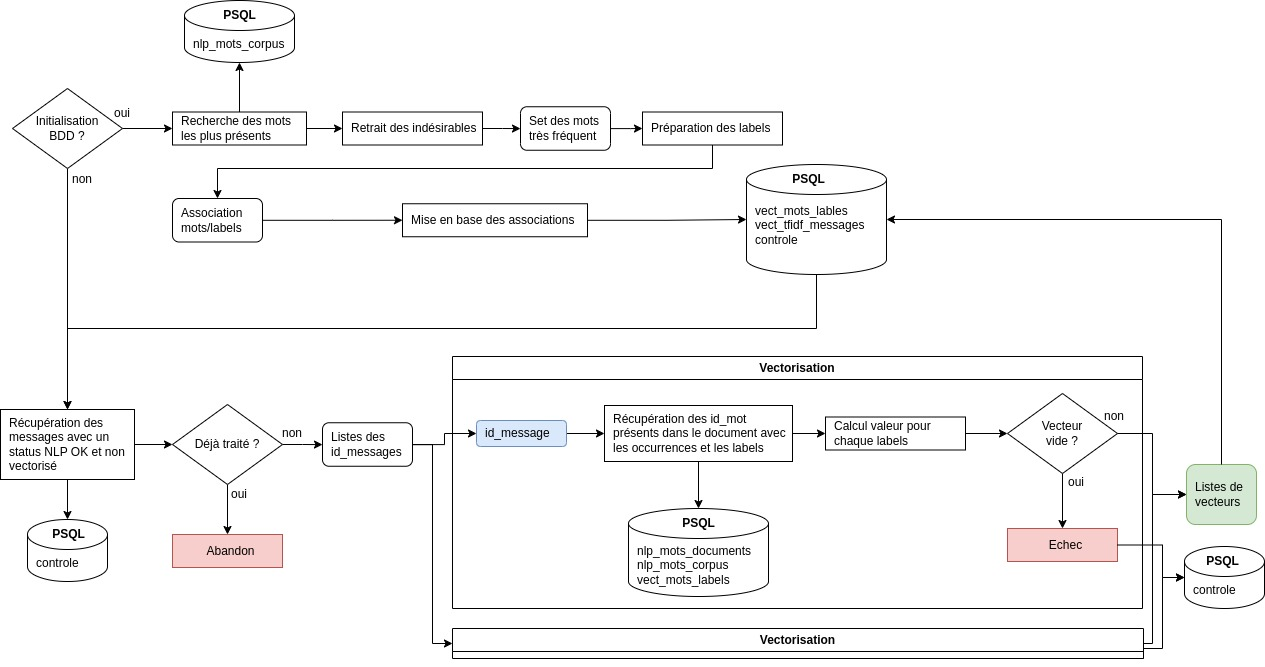
\includegraphics[width=\linewidth]{img/tfidf}
            \caption{Schéma de la vectorisation TFIDF}
            \label{fig:tfidf}
        \end{figure}

        Une fois la phase de récupération des mots faites, il a fallu sélectionner quels mots seront utilisés pour vectoriser les documents.
        J'ai décidé de me limiter sur un ensemble de mots les plus courants dans le corpus sous plusieurs critères :
        \begin{itemize}
            \item Les plus grandes fréquences dans le corpus
            \item Les plus grandes occurrences par catégorie
            \item les occurrences les plus importantes dans les documents d'une catégorie que dans l'autre
        \end{itemize}
        Ces mots sont récupérés via les commandes SQL suivantes :
        \begin{lstlisting}[title=Commandes SQL pour récupérer les mots les plus présent, language=SQL]
SELECT mot FROM nlp_mots_corpus ORDER by freq_corpus DESC;
SELECT mot FROM nlp_mots_corpus ORDER by freq_spam DESC;
SELECT mot FROM nlp_mots_corpus ORDER by freq_ham DESC;
SELECT mot FROM nlp_mots_corpus ORDER by freq_documents DESC;
SELECT mot FROM nlp_mots_corpus ORDER by freq_ham, freq_spam DESC;
SELECT mot FROM nlp_mots_corpus ORDER by freq_spam, freq_ham DESC;
SELECT mot FROM nlp_mots_corpus WHERE freq_ham >= 2*freq_spam ORDER BY freq_ham DESC;
SELECT mot FROM nlp_mots_corpus WHERE freq_spam >= 2*freq_ham ORDER BY freq_spam DESC;
SELECT mot, freq_ham/freq_spam as "ratio ham/spam" FROM nlp_mots_corpus WHERE freq_ham > 0 AND freq_spam > 0 ORDER BY "ratio ham/spam" DESC;
SELECT mot, freq_spam/freq_ham as "ratio spam/ham" FROM nlp_mots_corpus WHERE freq_ham > 0 AND freq_spam > 0 ORDER BY "ratio spam/ham" DESC;
        \end{lstlisting}
        Des \emph{LIMIT X} sont ajoutés à la fin de chaque instruction pour que conserver que les $X$ mots les plus importants.
        Certains mots très fréquents avec une connotation forte sur le dataset ont été retirés (spamassassinsightings, spamassassindevel)
        Le label de chaque mot est construit de la manière suivante, \emph{m\_<id\_mot>}.\\

        Chaque document sera vectorisé en fonction des mots retenus et uniquement avec les informations présentes dans les tables :
        \begin{itemize}
            \item nlp\_mots\_documents(occurrence) - fréquence du mot dans le document
            \item nlp\_mots\_corpus(freq\_documents) - nombre de documents du corpus contenant ce mot
            \item controle(nlp\_status) - count sur le nombre de documents ayant réussi le processus NLP
        \end{itemize}

        \paragraph{Choix techniques}
            Le choix de la vectorisation TFIDF a été décidé par sa proximité avec la distribution de Zipf qui est transposée en python dans ce projet.
            L'idée principale de cette vectorisation était d'avoir un minimum de mots dans la base vectorielle.
            Initialement, j'avais fixé une limite à 200 pour les requêtes SQL\@.
            Cela m'a généré une base d'environ 1200 mots.
            Le problème est que j'ai 5 messages qui ont terminé en vecteur null à la fin de la vectorisation.
            En basculant cette limite à 500 j'obtiens une liste de 2940 mots et tous les documents sont vectorisés.\\

            Le processus de vectorisation utilise également le module multiprocessing pour accélérer au maximum le traitement.
            L'insertion des vecteurs dans la base de données se fait itérativement par document.

        \paragraph{Base de données}
            Le schéma de la base de données pour la phase de vectorisation est montré dans la figure~\ref{fig:tfidf_bdd}.
            \begin{figure}[H]
                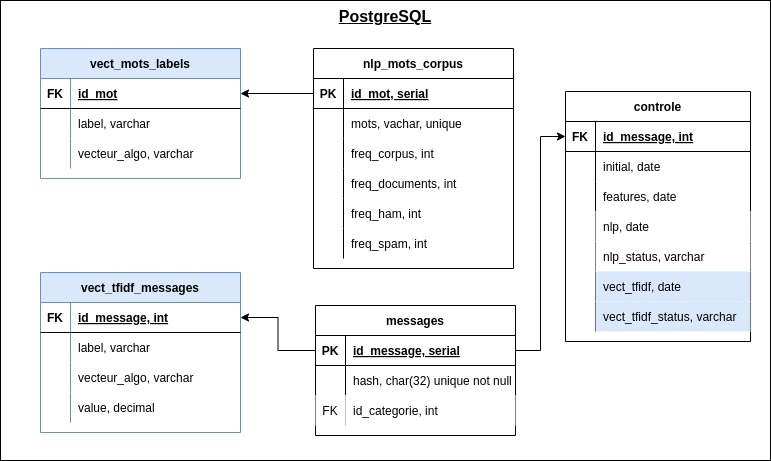
\includegraphics[width=\linewidth]{img/tfidf_bdd}
                \caption{Schéma de la vectorisation TFIDF}
                \label{fig:tfidf_bdd}
            \end{figure}

            Initialement, la table contenant les vecteurs devait avoir comme colonne les labels de chaque mot.
            Cependant, PSQL limite ses tables à 1600 colonnes.
            Ce format aurait dû permettre une intégration plus simple et plus rapide un dataframe pandas pour le traitement via IA\@.\\
            Les tables présentes dans la base sont :
            \begin{itemize}
                \item vect\_mots\_labels - contient la liste d'association entre les mots et les labels définis pour un type de vectorisation
                \item vect\_tfidf\_message - liste toutes les valeurs de la vectorisation par message et par label
                \begin{itemize}
                    \item id\_message
                    \item vecteur\_algo
                    \item label
                    \item value - valeur tfidf pour le message et pour le label
                \end{itemize}
            \end{itemize}
            Cette architecture est plus flexible pour l'ajout de nouvelle méthode de vectorisation.
            Seules les labels non null sont stockés dans la base.
            Cela implique que les labels manquants pour un message doivent être initialisés à 0 avant le début du traitement IA\@.
            La table \emph{vect\_mots\_labels} doit permettre de retrouver la liste complète des labels valident pour un vecteur.

        \paragraph{Analyse partielle}
            TODO
		\newpage

	\section{Modélisation}
		\label{sec:modelisation}
		\subsection{Entraînements}
\subsection{Validation}

		\newpage

	\section*{Conclusion}
		\label{sec:Conclusion}
		Avec ce projet nous avons vu le montage d'une infrastructure basée sur docker pour le stockage des informations récoltées et générées lors des différentes phases.
		Les fonctions développées pour les bases SQL et NoSQL sont utilisées dans toutes les phases de traitement.\\

		Faute de sources, il n'a pas été possible de mettre en place une automatisation pour la récupération des mails.
		Il a été nécessaire de les récupérer manuellement dans d'autres projet du même type.\\

		Le traitement initiale des mails est totalement automatisé grâce à Python et aux modules email et re.
		Ce nettoyage a permis de ne conserver que l'essentiel des corps de message tout en écartant les mails corrompu, sans texte, ou avec un mauvais encodage.\\

		Pour agrémenter notre jeux de données la recherche de caractéristique s'est concentré sur la forme des textes ainsi que sur la présence d'éléments non textuel.
		Les résultats de cette recherche n'a pas été aussi concluant que ce qui était espéré.\\

		La phase de traitement du langage visait à réduire les textes au minimum en tentant de conserver un maximum de sens.
		Pour cela, la lemmatisation semblait la meilleure option.
		Le modèle neuronale développer par StandfordNLP à permis de réaliser cette opération. \\

		Enfin la vectorisation a été réalisée en utilisant la méthode TF-IDF (Term Frequency - Inverse Document Frequency).
		Cette méthode est en accord avec l'idée d'analyse les mails en se basant sur la présence de certains mots.
		L'ensemble des documents pu être généré mais des ajustements ont du être fait pour ne pas avoir de vecteur null.

		Le tableau~\ref{tab:evolution} montre l'évolution du nombre de document et des mots au fur et à mesure des phases du projet
		\begin{table}[H]
            \centering
            \begin{tabular}{l|rrr]}
                Phase/Etape & nombre de documents & nombre de mots & nombre de mots uniques\\
                \hline
				Récolte & 5798 & 2385120 & 262614\\
				Transformation & 5658 & 1222793 & 99772\\
				Sauvegarde & 5333 & 1163550 & 99772\\
				Traitement du langage & 5333 & 658524 & 39947\\
				Vectorisation & 5333 & 453068 & 2942\\
            \end{tabular}
            \caption{Problèmes possibles avec la mise en base}
            \label{tab:evolution}
        \end{table}

		L'utilisation d'une Random Tree Forest a permis d'entrainer un modèle avec un résultat de 98\% sur la classification des document.
		Cependant, il convient de valider ce résultat sur des messages n'ayant encore jamais été vu par Errol

	\newpage
	\appendix
	\section{Développement visualisation distribution de Zipf}
		\label{sec:devZipf}
			\paragraph{Présentation}
		La loi de distribution de Zipf est une loi empirique (basée sur l'observation) qui veut que le mot le plus fréquent est, à peu de chose près, 2 fois plus fréquent que le $2^{eme}$, 3 fois plus fréquent que le $3^{eme}$ etc.\\

		La formulation finale de la $1^{ere}$ loi de Zipf est la suivante :

		\begin{align*}
				|mot| = constante \times rang(mot)^{k \approx 1}
		\end{align*}

		avec \emph{$|mot|$} la fréquence d'apparition d'un mot, \emph{constante} une valeur propre à chaque texte, \emph{rang(mot)} la place du mot dans le tri décroissant par fréquence d'apparition et \emph{k} un coefficient proche de 1. 

	\paragraph{Développement}
		Afin de pouvoir utiliser les résultats de cette distribution dans ce projet, j'ai développé un ensemble de fonctions sur un corpus "\emph{reconnu}". Mon choix s'est porté sur le corpus \emph{Brown} (voir \ref{Brown_corpus}) présent dans la librairie \emph{nltk}. Ce corpus contient environ 500 documents contenant 1 millions de mot en anglais.\\

		Le processus d'analyse se fait sur 2 versions de ce corpus.
		\begin{itemize}
			\item la première version contient tous les mots sans modifications
			\item le seconde version contient tous les mots sans les \emph{stopwords}
		\end{itemize}
		Les \emph{stopwords} sont des mots qui n'ont pas ou peu de signification dans un texte. Ces mots sont retirés dans la $2^e$ version pour voir l'effet d'une réduction sur la distribution de Zipf. \\

		Les paragraphes ci-dessous détaillent les étapes du développement :

		\subparagraph{Étape 1 - Ordonner les mots}
			La première étape est de compter les occurrences de tous les mots des 2 corpus et de les ranger en fonction de leur nombre d’occurrence. 
			\begin{lstlisting}[title=Triage des mots]
def frequence_mot(bag, freq=None):
    """
    Calcule la frequence de chaque mot dans un sac de mot
    :param bag: <list> - liste de tous les mots d'un texte
    :param freq: <dict> - dictionnaire avec {<str> mot: <int> frequence}
    :return: <dict> - dictionnaire avec la frequence par mot {mot: frequence}
    """
    if freq is None:
        freq = {}
    for mot in bag:
        freq[mot] = freq.get(mot, 0) + 1
    return freq

def classement_zipf(dico):
    """
    Trie un dictionnaire de mots : occurence et leur assigne un rang en fonction du nombre d'occurence
    :param dico: <dict> dictionnaire de mot: occurrences
    :return: <list> {"rang": <int>, "mot": <str>, "frequence": <int>}
    """
    ranked = []
    for rang, couple in enumerate(sorted(dico.items(), key=lambda item: item[1], reverse=True), start=1):
        ranked.append({"rang": rang,
                       "mot": couple[0],
                       "frequence": couple[1]})

    return ranked \end{lstlisting}


    		On obtient les représentations suivantes: 
		\begin{figure}[H]
				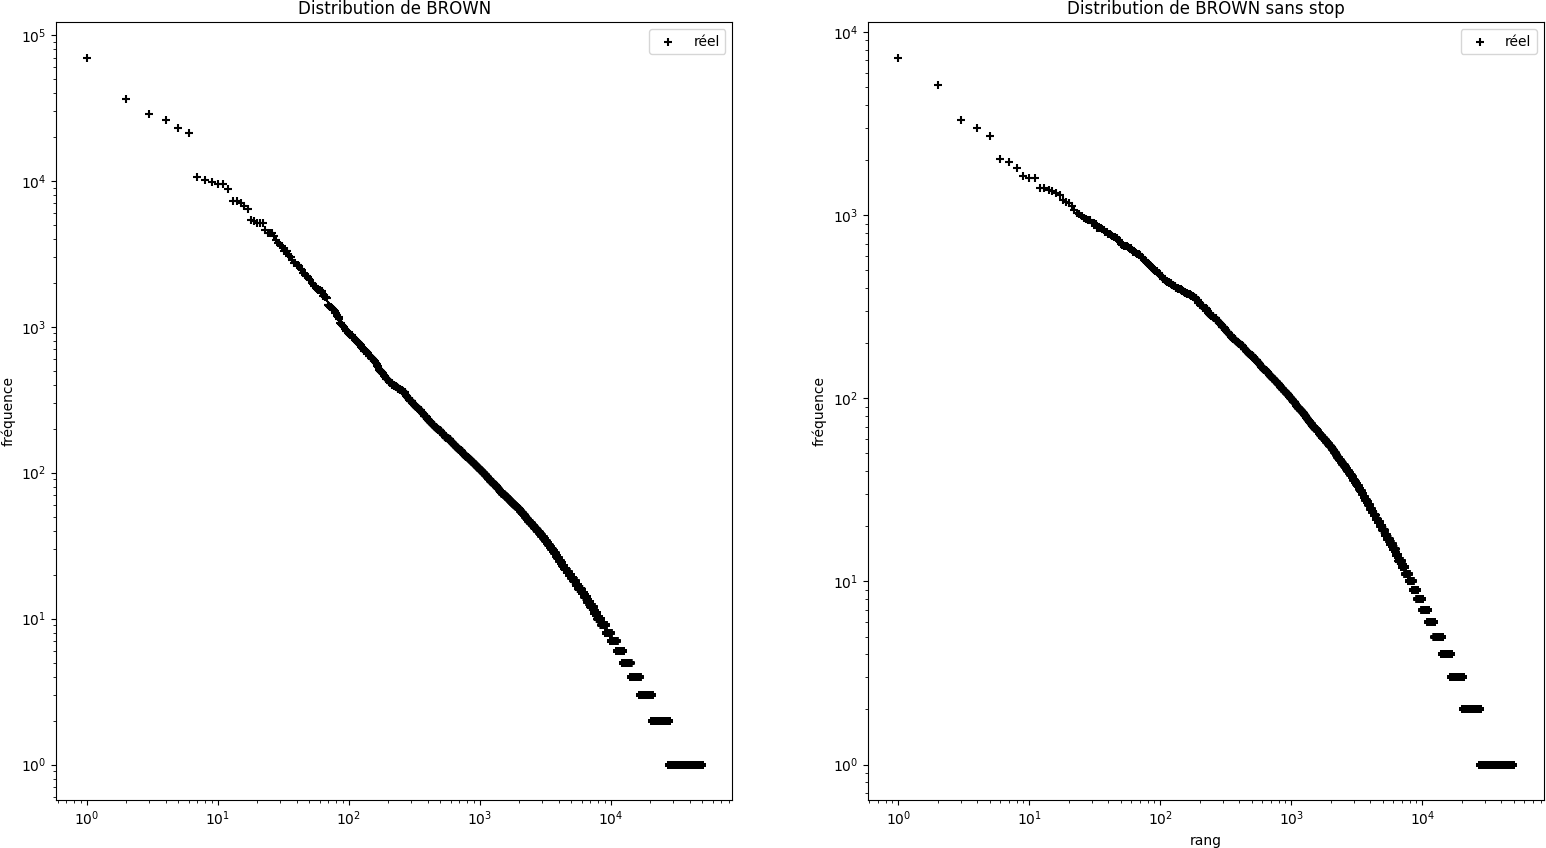
\includegraphics[width=\linewidth]{img/distribZipf.png}
				\caption{Distribution de Zipf pour les deux corpus}
		\end{figure}    		

    		\begin{itemize}
    			\item Nombre de mots dans brown:	mots: 49398	occurences: 1012528
    			\item Nombre de mots dans brown stop:	mots: 49383	occurences: 578837\\
    		\end{itemize}

    		La distribution de la version complète du corpus semble à première vue plus fidèle à la représentation classique de la distribution de Zipf. 

		\subparagraph{Etape 2 - calcul de la constante}
			Le premier paramètre qu'il faut déterminer est la \emph{constante}. Pour ce faire j'effectue le calcul suivant pour tous les mots :

			\begin{align*}
				constante = |mot| \times rang(mot)
			\end{align*}

			On obtient une liste de toutes les constantes théoriques pour chaque mot selon son rang.
			De cette liste, nous allons extraire la moyenne et la médiane.

			\begin{figure}[H]
				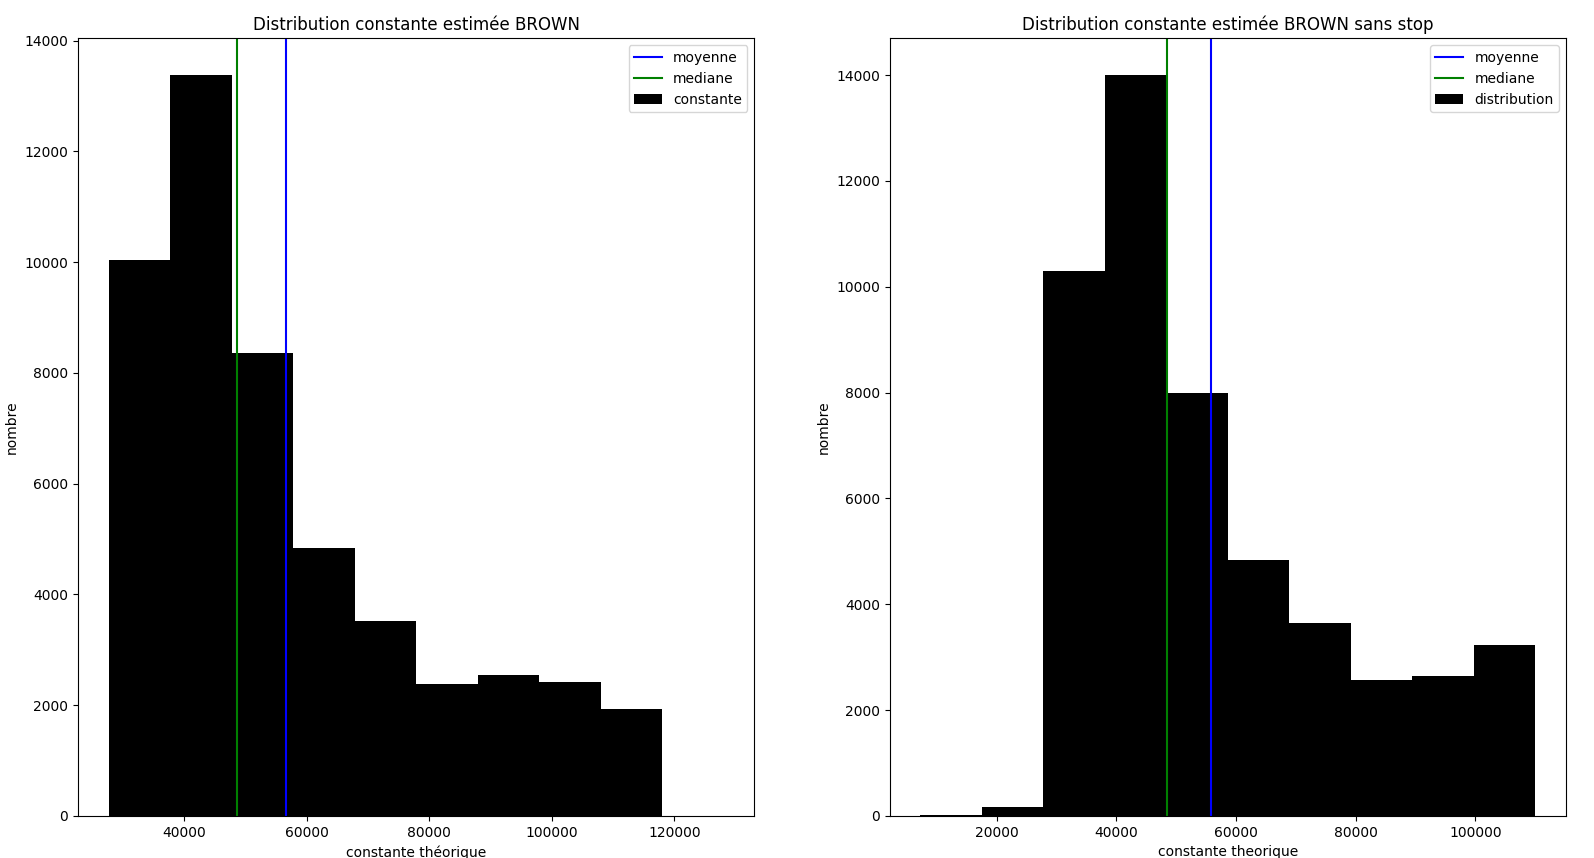
\includegraphics[width=\linewidth]{img/distribContTh.png}
				\caption{Distribution des constantes théoriques pour les deux corpus}
			\end{figure}

			On voit qu'il y a une majorité de mots donnant une constante brute comprise entre $20.000$ et $60.000$. Dans les deux corpus
			La différence entre les moyennes et médianes des deux corpus n'est pas flagrante :
			\begin{itemize}
				\item Brown moyenne: 56525.81, médiane: 48601.50
				\item Brown (- stopwords) moyenne: 55809.97, médiane: 48494.00
			\end{itemize}


		\subparagraph{Etape 3 - recherche du coefficient}
			Le coefficient $k$ permet d'ajuster le résultat, et pourra éventuellement donner une indication de complexité. La recherche de $k$ se fera sur les deux corpus avec utilisant les moyennes et médianes.\\

			Pour ce faire nous allons:

			\begin{enumerate}
				\item Faire la liste de tous les coefficients possibles dans l'intervalle $[0.86, 1.3]$ avec un pas de $0.01$\footnote{les bornes et le pas sont totalement arbitraire afin d'obtenir un graphique présentable}.
				\item Calculer toutes la fréquences théoriques de tous les rangs avec tous les coefficients possibles en utilisant les constantes moyenne et médiane de chaque corpus.
				\item Calculer la moyenne des coûts absolus entre les fréquences théoriques par coefficient avec la fréquence réelle observée pour chaque corpus.\\
			\end{enumerate}

			Le couple coefficient/constante avec le coup minimal sera retenu pour l'utilisation dans la phase de \emph{feature engineering}. \\	

			\begin{lstlisting}[title=Fonctions utilisées dans la recherche du coefficient]
def zipf_freq_theorique(constante, rang, coef):
    """
    Calcul la frequence theorique d'un mot selon son rang, la constante du texte et un coeficiant d'ajustement
    :param constante: <int> constante determinee par la distribution de Zipf
    :param rang: <int> rang du mot selon sa frequence
    :param coef: <float> variable d'ajustement
    :return: <float> frequence theorique zipfienne
    """
    return constante / (rang ** coef)

def cout(l1, l2, methode):
    """
    Calcul le cout de l'ecart entre les elements de l1 et le l2, place par place
    :param l1: <list> liste d'entier
    :param l2: <liste> liste d'entier
    :param methode: <str> methode de calcul du cout
    :return: <float> cout selon methode
    """
    if len(l1) != len(l2):
        print("Erreur, fonction cout: l1 & l2 de taille differente", file=sys.stderr)
        return None

    if len(l1) == 0:
        print("Erreur, fonction cout: liste vide", file=sys.stderr)

    if methode.lower() not in ['absolue', 'carre', 'racine']:
        print("Erreur, fonction cout - methode '{}' inconnue".format(methode), file=sys.stderr)
        return None

    if methode.lower() == 'absolue':
        return np.mean([abs(x-y) for x, y in zip(l1, l2)])

    if methode.lower() == 'carre':
        return np.mean([(x-y)**2 for x, y in zip(l1, l2)])

    if methode.lower() == 'racine':
        return np.sqrt(np.mean([(x-y)**2 for x, y in zip(l1, l2)]))

    return None\end{lstlisting}

			\begin{lstlisting}[title=Calcul des fréquences par coefficient]
    ls_coef = list(np.arange(0.86, 1.3, 0.01))
    zbmo_th = {coef: [stats.zipf_freq_theorique(zb_const_moyen, r, coef) for r in zb_rang] for coef in ls_coef}
    zbme_th = {coef: [stats.zipf_freq_theorique(zb_const_median, r, coef) for r in zb_rang] for coef in ls_coef}
    zbmoth_cmoy = [stats.cout(zb_freq, zbmo_th[coef], 'absolue') for coef in ls_coef]
    zbmeth_cmoy = [stats.cout(zb_freq, zbme_th[coef], 'absolue') for coef in ls_coef]

    zbsmo_th = {coef: [stats.zipf_freq_theorique(zbs_const_moyen, r, coef) for r in zbs_rang] for coef in ls_coef}
    zbsme_th = {coef: [stats.zipf_freq_theorique(zbs_const_median, r, coef) for r in zbs_rang] for coef in ls_coef}
    zbsmoth_cmoy = [stats.cout(zbs_freq, zbsmo_th[coef], 'absolue') for coef in ls_coef]
    zbsmeth_cmoy = [stats.cout(zbs_freq, zbsme_th[coef], 'absolue') for coef in ls_coef] \end{lstlisting}

		La recherche du coefficient nous retourne les éléments suivants:
			\begin{figure}[H]
				\includegraphics[width=\linewidth]{img/coutZipf.png}
				\caption{Coût absolu moyen par coefficient}
			\end{figure}

			\begin{itemize}
				\item Coût min brown moyenne: 5.93, median: 7.01
				\item Coût min brown (- stopwords) moyenne: 6.95, median: 6.46
				\item Coefficient min brown moyenne: 0.92, median: 0.91
				\item Coefficient min brown (- stopwords) moyenne: 0.97, median: 0.95
			\end{itemize}

	\paragraph{Résultats}

		Le tableaux ci dessous rappelle les données récupérées au long de la recherche:
		\begin{center}
			\begin{tabular}{|l|c|c|}
				\hline
				& BROWN avec stopwords & BROWN sans stopwords \\
				\hline
				nombre de mots uniques & 49398 & 49383 \\
				\hline
				nombre de mots total & 1012528 & 578837 \\
				\hline
				Constante moyenne & 56525.81 & 55809.97 \\
				\hline
				Constante médiane & 48601.50 & 48494.00 \\
				\hline
				Coefficient avec moyenne & 0.92 & 0.97 \\
				\hline
				Cout du coefficient moyenne & 5.93 & 6.95 \\
				\hline
				Coefficient avec médiane & 0.91 & 0.95 \\
				\hline
				Cout du coefficient médiane & 7.01  & 6.46 \\
				\hline
			\end{tabular}		
		\end{center}

		D'après les données il est possible de dire que l'on obtient de meilleurs résultats si on conserve tous les mots du corpus. Dans ce cas l'utilisation de la moyenne des constantes génère un taux d'erreur plus faible que la médiane.\\

		Ci-dessous la représentation des fréquences théoriques avec le coefficient optimal pour chaque corpus et chaque méthode. On voit que la courbe de la constante moyenne sur le corpus brute est celle qui suit le mieux les données réelles.
		\begin{figure}[H]
			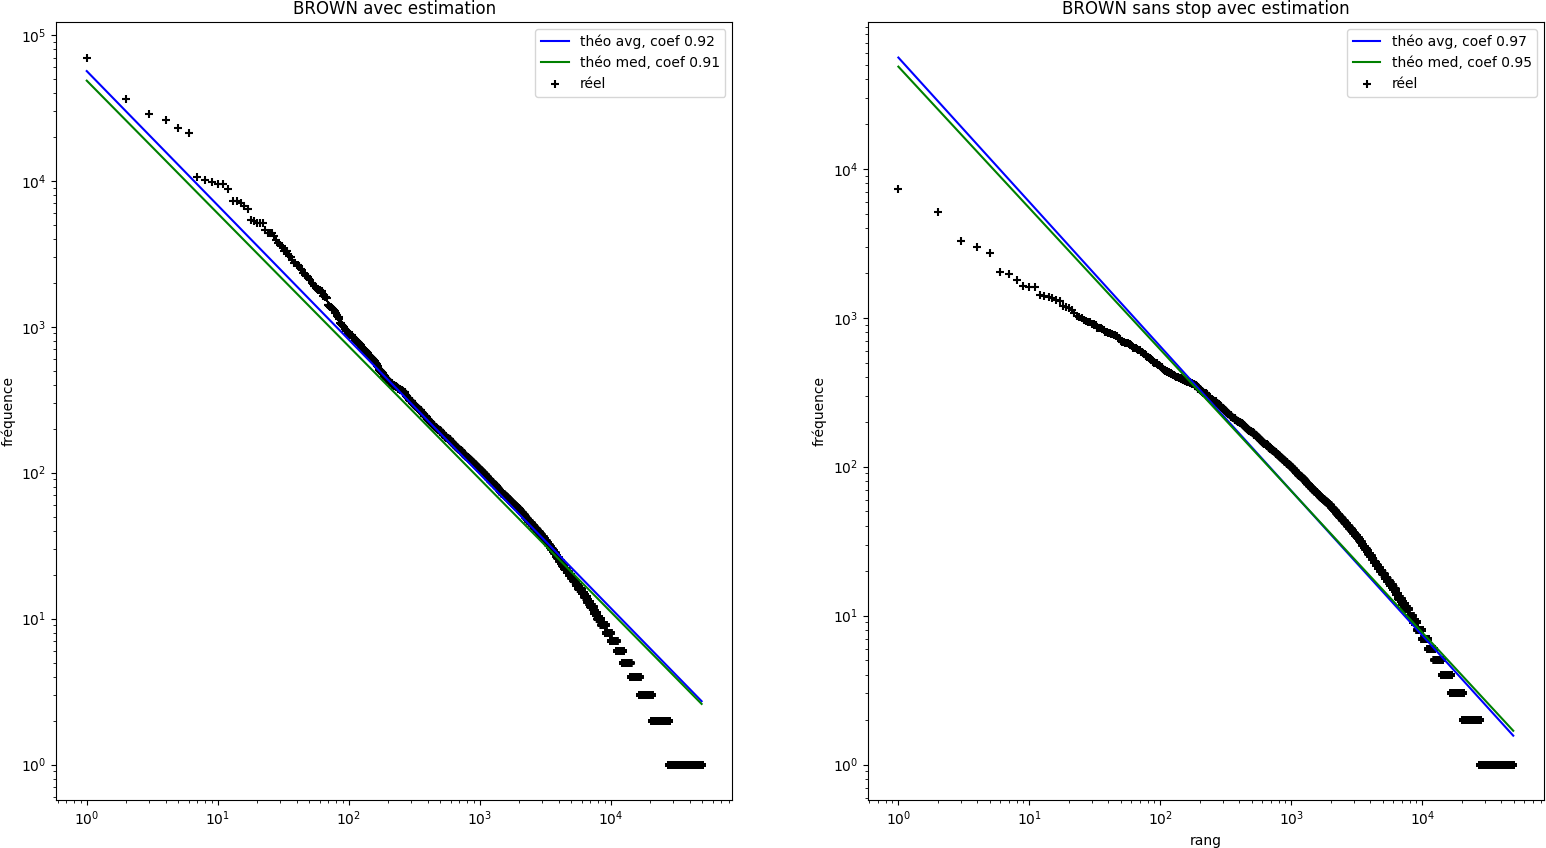
\includegraphics[width=\linewidth]{img/zipfFin.png}
			\caption{Distribution de Zipf avec les estimations}
		\end{figure}

		En conclusion, j'utiliserais la moyenne des constantes sur un document complet afin de déterminer le coefficient dans ma recherche de spam.
	\newpage

	\section{Modèles}
		\label{sec:modeles}
				\subsection{Naïves Bayes}
			Ce type de modèle est utilisé par le module \emph{langdetect} qui me sert pour la détection des langues.

			\paragraph{Introduction}
				Les modèles Naïves Bayes se basent sur le théorème de probabilité de Bayes. Il permet de déterminer la probabilité conditionnelle d'apparition d'un évènement A sachant qu'un évènement B s'est produit. Le terme naïf fait référence au fait que l'on présuppose que les évènements A et B ne sont pas corrélés.\\
				Ces techniques sont utilisées pour des modèles de classification en apprentissage supervisé.\\

				La formule mathématique de ce théorème est la suivante :
				\begin{eqnarray}\label{NBeq}
					P(A|B) &=& \frac{P(B|A)P(A)}{P(B)}
				\end{eqnarray}

			On recherche ici $P(A|B)$, c'est a dire la probabilité d'apparition d'un évènement A sachant que l'évènement B s'est produit. \\ 

			Pour ce faire nous avons besoin des données suivantes :
			\begin{itemize}
				\item $P(B|A)$ est la probabilité que l'évènement B s'est produit sachant que l'évènement A s'est produit
				\item $P(A)$ est la probabilité d'apparition de l'évènement A
				\item $P(B)$ est la probabilité d'apparition de l'évènement B
			\end{itemize}

			\paragraph{Exemples d'utilisation}
				Les exemples ci dessous vont permettre d'illustrer l'utilisation de cette technique. D'abord manuellement sur un petit jeu de données puis à l'aide d'un code pré-existant sur un autre jeu de données plus important.

				\subparagraph{Manuel}
					Dans cet exemple nous allons déterminer la probabilité qu'a un joueur d'aller sur le terrain selon les conditions météorologiques. Cette probabilité sera calculée en fonction des données récupérées lors des matchs précédents.\footnote{Les données présentées sont inventées} \\

					On recherchera ainsi la probabilité de présence sur le terrain d'un joueur selon la météo $P(A|B)$. Pour ce faire nous auront besoin de: 
					\begin{itemize}
						\item $P(A)$ Probabilité de jouer quelque soit le temps
						\item $P(B)$ Probabilité de l'évènement météorologique
						\item $P(B|A)$ Probabilité de l'évènement sachant que le joueur a été sur le terrain					
					\end{itemize}

				\begin{table}[H]
					\centering
					\captionof{table}{Données de présence sur le terrain} \label{tab:data}
					\begin{tabular}{|l|c|c|c|c|c|c|c|}
						\hline
						météo & soleil & soleil & couvert & pluie & pluie & pluie & couvert \\
						\hline
						présent & non & non & oui & oui & oui & non & oui \\
						\hline
						\hline
						météo & soleil & soleil & pluie & soleil & couvert & couvert & pluie \\
						\hline
						présent & non & oui & oui & oui & oui & oui & non \\
						\hline
					\end{tabular}
				\end{table}

				\begin{table}[H]
					\centering
					\captionof{table}{Synthèse et probabilité simple P(A) et P(B)} \label{tab:pab}
					\begin{tabular}{|l|c|c|r|}
						\hline
						météo & oui & non & $P(B)$\\
						\hline
						couvert & 4 & 0 & $4/14$\\
						\hline
						soleil & 2 & 3 & $5/14$\\
						\hline
						pluie & 3 & 2 & $5/14$\\
						\hline
						$P(A)$ & $9/14$ & $5/14$ & \\
						\hline
					\end{tabular}
				\end{table}

				On peut déterminer les probabilités de chaque météo en fonction de la présence du joueur sur le terrain P(B|A). Pour ce faire on divise le nombre d'évènements de présence du joueur lors d'un évènement météo par le nombre total d'évènements de présence du joueur

				\begin{table}[H]
					\centering
					\captionof{table}{Probabilité météo selon présence du joueur} \label{tab:pba}
					\begin{tabular}{|l|c|c|}
						\hline
						météo & P(B|oui) & P(B|non) \\
						\hline
						couvert & $4/9$ & $0/5$ \\
						\hline
						soleil & $2/9$ & $3/5$ \\
						\hline
						pluie & $3/9$ & $2/5$ \\
						\hline	
					\end{tabular}
				\end{table}

				On va maintenant calculer la probabilité qu'à un joueur d'être sur le terrain si le temps est couvert.\\
				On commence par la probabilité du oui:
				\begin{eqnarray*}
					P(A|B) &=& \frac{P(B|A)P(A)}{P(B)}\\
					P(A|B) &=& \frac{\frac{4}{9}\cdot\frac{9}{14}}{\frac{4}{14}}\\
					P(A|B) &=& \frac{\frac{4}{14}}{\frac{4}{14}}\\
					P(A|B) &=& \frac{4}{14}\cdot\frac{14}{4}\\
					P(A|B) &=& 1
				\end{eqnarray*}

				On enchaîne sur la probabilité de ne pas jouer si le temps est couvert
				\begin{eqnarray*}
					P(A|B) &=& \frac{P(B|A)P(A)}{P(B)}\\
					P(A|B) &=& \frac{\frac{0}{5}\cdot\frac{5}{14}}{\frac{4}{14}}\\
					P(A|B) &=& 0\cdot\frac{14}{4}\\
					P(A|B) &=& 0
				\end{eqnarray*}	

				On peut dire que si le temps est couvert le joueur très probablement sur le terrain			 
				On peut également déterminer la probabilité de jouer pour chaque évènement météo
				\begin{table}[H]
					\centering
					\captionof{table}{Probabilité présence du joueur selon la météo} \label{tab:pab2}
					\begin{tabular}{|l|c|c|c|}
						\hline
						météo & oui & non & plus probable\\
						\hline
						couvert & 1 & 0 & oui\\
						\hline
						soleil & 2/5 & 3/5 & non \\
						\hline
						pluie & 3/5 & 2/5 & oui \\
						\hline
					\end{tabular}
				\end{table}

				\emph{Cas polynomial}: Il est possible de déterminer la probabilité d'un évènement par rapport à plus autres. Dans ce cas, il faudra multiplier entre elles les probabilités de ces évènements selon l'apparition de l'évènement voulu.\\

				 Calcul pour un évènement (A) selon 2 autres évènements (B et C)
				 \begin{eqnarray*}
				 	P(A|BC) &=& \frac{P(B|A)P(C|A)P(A)}{P(B)P(C)}
				 \end{eqnarray*}

				\subparagraph{En code} Dans cet exemple nous allons utiliser un code existant dans la librairie python scikit-learn\cite{scikit-learn}. Ce moteur Naïves Bayes va nous permettre cette fois-ci de catégoriser des variétés d'iris selon la longueur et la largeur des pétales et des sépales. Les données proviennent cette fois-ci d'un dataset également disponible dans scikit-learn.

				Nous allons utilisé le modèle \emph{GaussianNB} de scikit-learn qui est adapté lorsque les données utilisées suivent une distribution normale. Ce qui semble être le cas pour les longueurs et largeur des sépale. 
				\begin{figure}[H]
					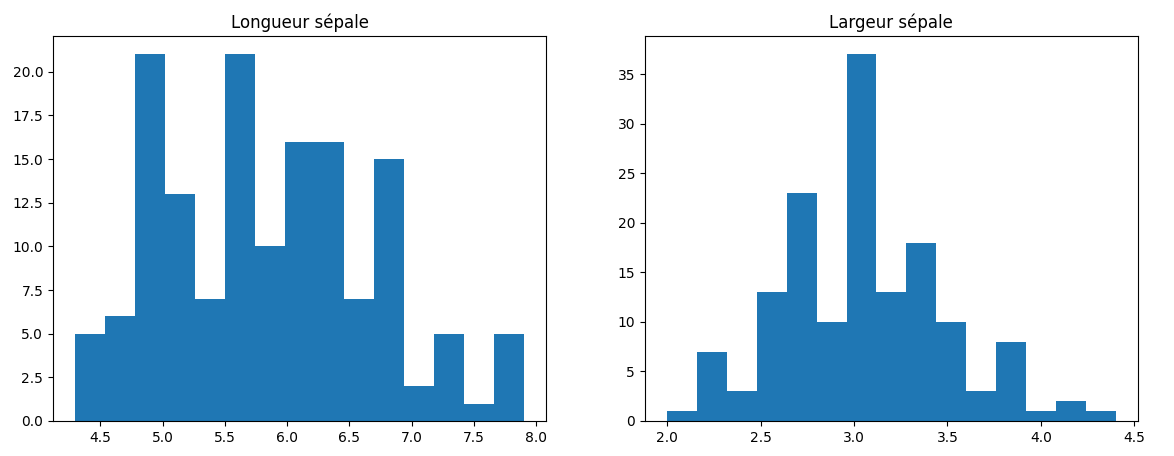
\includegraphics[width=\linewidth]{img/NBdistrib.png}
					\caption{Distribution des longueurs et largeurs des sépales}
				\end{figure}

\begin{lstlisting}[title=Progamme complet]
from sklearn.datasets import load_iris
from sklearn.model_selection import train_test_split
from sklearn.naive_bayes import GaussianNB
from sklearn.metrics import accuracy_score, confusion_matrix, ConfusionMatrixDisplay, f1_score, \
    recall_score

import matplotlib.pyplot as plt

X, y = load_iris(return_X_y=True)

X_train, X_test, y_train, y_test = train_test_split(X, y, test_size=0.33, random_state=0)
model = GaussianNB()
model.fit(X_train, y_train)

y_pred = model.predict(X_test)
precision = accuracy_score(y_pred, y_test)
recall = recall_score(y_test, y_pred, average="weighted")
f1 = f1_score(y_pred, y_test, average="weighted")

print("Precision:", precision)
print("Rappel:", recall)
print("Score F1:", f1)

plt.figure('Donnees du modele', figsize=(14, 5))
plt.subplot(1, 3, 1, title='Donnees du train set')
plt.scatter(X_train[:, 0], X_train[:, 1], c=y_train)
plt.xlabel('Sepale long.')
plt.ylabel('Sepale larg.')
plt.subplot(1, 3, 2, title='Donnees du test set')
plt.scatter(X_test[:, 0], X_test[:, 1], c=y_test)
plt.xlabel('Sepale long.')
plt.subplot(1, 3, 3, title='Donnees test apres evaluation')
plt.scatter(X_test[:, 0], X_test[:, 1], c=y_pred)
plt.xlabel('Sepale long.')
plt.show()

cm = confusion_matrix(y_test, y_pred, labels=[0, 1, 2])
disp = ConfusionMatrixDisplay(confusion_matrix=cm, display_labels=[0, 1, 2])
disp.ax_.set_title('Matrice de confusion')
disp.plot()
plt.show()

plt.figure('Distribution des donnees Iris', figsize=(14, 5))
plt.subplot(1, 2, 1, title='Longueur sepale')
plt.hist(X[:, 0], bins=15)
plt.subplot(1, 2, 2, title='Largeur sepale')
plt.hist(X[:, 1], bins=15)
plt.show()\end{lstlisting}

				Les données du dataset ont été séparés en 2 jeux, un pour l’entraînement du modèle et un pour le test. On obtient alors la représentation suivantes après entrainement et test du modèle
				\begin{figure}[H]
					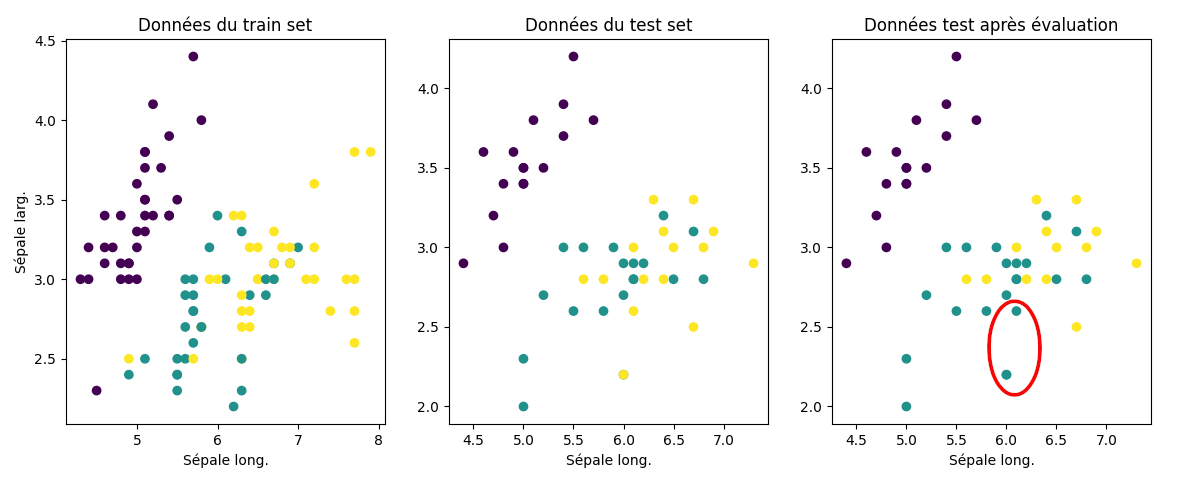
\includegraphics[width=\linewidth]{img/NBdata.png}
					\caption{Représentation des données }
				\end{figure}

				Dans les données de test nous avons 2 catégorisations qui n'ont pas été réalisées correctement. On obtient les scores suivants :
				\begin{itemize}
					\item Précision: 0.96                    \footnote{La précision est la proportion des éléments correctement identifiés sur l'ensemble des éléments prédit}
					\item Rappel: 0.96						\footnote{Le rappel est la proportion des éléments correctement identifiés sur l'ensemble des éléments de la catégorie}
					\item Score F1: 0.9604285714285714		\footnote{Le Score F1 est la moyenne harmonique calculée de la manière suivante $2*(precision*rappel)/(precision+rappel)$}
				\end{itemize}				

				\begin{figure}[H]
					\centering
					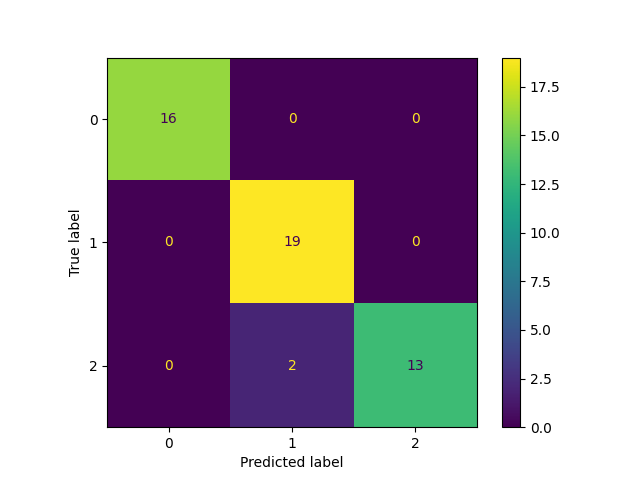
\includegraphics[scale=0.7]{img/NBmatrix.png}
					\caption{Matrice de confusion}
				\end{figure}

				A l'aide de ce modèle nous devrions avoir une 96\% de chance de déterminer la bonne variété d'iris en se basant sur la longueur et la largeur des sépales.  

			\paragraph{Avantages et inconvénients} 
				Le modèle Naïve Bayes est un modèle simple et rapide qui ne nécessite pas de grande capacités de calcul. De ce fait il permet de traiter une grande quantité de données.\\

				Cependant, les données qui lui sont fournies ne doivent pas être corrélées ce qui est rarement le cas dans les problèmes du monde réel. Ce type de modèle est limité à des problèmes de classification supervisée. Si on se fie à l'équation (\ref{NBeq}) la probabilité d'apparition de l’évènement B : P(B) ne peut pas être nulle.
	\newpage

	\section{Bibliographie}
		\label{sec:bibliographie}
		\bibliographystyle{plain}
		\bibliography{IED_Lang_fouille}
	\newpage


	\section{Sitotec}
		\subsection{Corpus}
			\begin{itemize}
				\item Enron company mails, fichier CSV contenant l'ensemble des mails d'une entreprise ayant fermée ses portes (33.834.245 mails) [en ligne], \url{https://www.kaggle.com/wcukierski/enron-email-dataset} (consulté le 27/01/2022) \label{Enron_dataset}
				\item Mails project SpamAssassin, projet opensource de détection de spam (6065 fichiers email déjà trier en ham et spam) [en ligne], \url{https://spamassassin.apache.org/old/publiccorpus/} (consulté le 27/01/2022) \label{SpamAssassin_dataset}
				\item Brown corpus, ensemble de texte en anglais publié en 1961 qui contient plus d'un million de mots \url{https://www.nltk.org/book/ch02.html} (consulté le 20/08/2022) \label{Brown_corpus}
				\item Spam generated by LLM, fichier csv avec des mail généré par IA \url{https://www.kaggle.com/datasets/trainingdatapro/generated-e-mail-spam} (consulté le 06/08/2024) \label{spamLLM}
			\end{itemize}
		
		\subsection{Modules}
			\begin{itemize}
				\item Page Github du projet \emph{langdetect} capable de différencier 49 langages avec une précision de 99\%, [en ligne] \url{https://github.com/Mimino666/langdetect} (consulté le 04/12/2022) \label{langdetect}
				\item Language Detection Library, présentation du module (anglais) [en ligne] \url{https://www.slideshare.net/shuyo/language-detection-library-for-java} (consulté le 04/12/2022)
				\item Suite de cours et de ressources en ligne pour comprendre MongoDB et réussi a faire la connexion avec un programme Python; [en ligne] \url{https://learn.mongodb.com/learning-paths/mongodb-python-developer-path} (consulté le 09/2023)
				\item Documentation de la librairie standard python sqlite [en ligne] \url{https://docs.python.org/3/library/sqlite3.html} (consulté le 09/2023)
				\item Documentation de la librairie psycopg2 [en ligne] \url{https://pypi.org/project/psycopg2/} (consulté le 09/2023)
				\item Documentation de la librairie sqlalchemy [en ligne] \url{https://docs.sqlalchemy.org/en/20/index.html} (consulté le 09/2023)
			\end{itemize}
			
		\subsection{Modèles}
			\paragraph{Naïves Bayes}
				Le modèle Naïves Bayes est employé dans le module langdetect (\ref{langdetect})
				\begin{itemize}
					\item Les algorithmes de Naïves Bayes, Explication sommaire du principe de ces type d'algorithme, [en ligne] \url{https://brightcape.co/les-algorithmes-de-naives-bayes/} (consulté le 26/03/2023)
					\item Naive Bayes Classification Tutorial using Scikit-learn, exemple d'utilisation de ce type de modèle avec python (anglais) [en ligne] \url{https://www.datacamp.com/tutorial/naive-bayes-scikit-learn} (consulté le 26/03/2023)
					\item Scikit learn Naive Bayes, description des types d'algorithme disponibles dans le module Scikitlearn en python (anglais) [en ligne] \url{https://scikit-learn.org/stable/modules/naive_bayes.html} (consulté le 26/03/2023)
				\end{itemize}

			\paragraph{Random Tree Forest}
				Le modèle Random Tree Forest est utilisé dans la section~\ref{sec:modelisation}
				\begin{itemize}
					\item Formules mathématiques utilisées dans SciKit learn [en ligne] \url{https://scikit-learn.org/stable/modules/tree.html#tree-mathematical-formulation} (consulté le 06/08/2024)
				\end{itemize}

	\section{Code Source}
		\subsection{GitHub}
			L'ensemble du code est disponible dans mon repository GitHub. \url{https://github.com/peredur0/errol}
	
\end{document}





















